% vim:nojs:spelllang=en_us tw=76 sw=4 sts=4 fo+=awn fmr={-{,}-} et ts=8
\documentclass[11pt,titlepage,twoside]{report}
%{-{1 Packages
\usepackage[T1]{fontenc}
\usepackage[utf8]{inputenc}
\usepackage{textcomp}

\usepackage{hevea}
\usepackage[subdir=samples,
            prefix=tutorial,
            ext=.zls,
            prompt={aneto.local:\ },
            compiler={../compiler/zeluc.byte},
            compilerflags={-I ../lib -I ./samples},
            lastflags={-i},
            includecmd={},
            html={../tools/zltohtml},
           ]{runverbatim}
\fvset{xleftmargin=3mm}
\ifhevea
\relax
\else
\runverbatimsetup{errstyle={formatcom=\small}}
\fi

\newcommand{\zls}[1]{\texttt{#1}}
\newcommand{\zlsmsg}[1]{\texttt{#1}}

\usepackage{a4wide}
\usepackage{alltt}
\usepackage{graphicx}
\usepackage{epsf}
\usepackage{amssymb}
\usepackage{hyperref}
\usepackage{cleveref}

\crefname{figure}{figure}{figures}

\usepackage[inline]{enumitem}
\newlist{inparaenum}{enumerate*}{1}
\setlist[inparaenum,1]{label=(\arabic*),ref=\arabic*}
\newenvironment{flatitemize}
  {\begin{itemize}[leftmargin=*]}
  {\end{itemize}}

%BEGIN IMAGE
\usepackage{tikz}
\usetikzlibrary{positioning,chains,matrix,shapes.arrows,scopes,
                shapes.misc,arrows,automata,calc,decorations.markings,
                decorations.text}
%END IMAGE

%}-}1
%{-{1 Macros

\ifhevea
\newcommand{\footnoteurl}[2]{\ahref{#2}{#1}}
\else
\newcommand{\footnoteurl}[2]{{#1}\footnote{\url{#2}}}
\fi


\newcommand{\f}{$f$}
\renewcommand{\t}{$t$}
\newcommand{\nil}{$\mathit{nil}$}

\newcommand{\cvode}{{\sc CVODE}}
\newcommand{\ly}{\ensuremath{\mathit{ly}}}
\newcommand{\lx}{\ensuremath{\mathit{lx}}}
\newcommand{\step}{\ensuremath{\mathit{step}}}
\newcommand{\init}{\ensuremath{\mathit{init}}}
\newcommand{\encore}{\ensuremath{\mathit{encore}}}
\newcommand{\field}{\ensuremath{\mathit{field}}}
\newcommand{\method}{\ensuremath{\mathit{method}}}

\newcommand{\rulename}[1]{{\small\sc ({#1})}}

\newcommand{\Solve}[2]{\mathit{solve}({#1})({#2})}

\newcommand{\Ifthenelse}[3]
   {\mathit{if}\,{#1}\,\mathit{then}\,{#2}\,\mathit{else}\,{#3}}

%\everymath{\displaystyle}
%\tikzstyle{block} = [draw,fill=blue!20,minimum size=1.5em]
%\tikzstyle{signal} = [draw,-latex,thick]
%\tikzstyle{jump over} = [{to path={-- ([yshift=-.7mm]\tikztostart |- #1)
%                          arc(-90:90:.7mm) |- (\tikztotarget)}}]

% see: 
% http://tex.stackexchange.com/questions/6135/how-to-make-beamer-overlays-with-tikz-node
\begin{latexonly}
\tikzset{onslide/.code args={<#1>#2}{%
  \only<#1>{\pgfkeysalso{#2}} % \pgfkeysalso doesn't change the path
}}

\tikzset{dimmedmarker/.code args={<#1> then <#2>}{%
  \alt<#1,#2>
  {
    \tikzstyle{marker} = [draw]
    \alt<#2>
    {\pgfkeysalso{->,red!80,draw opacity=.15}}
    {\pgfkeysalso{->,red!80,draw opacity=.50}}
  }
  {
    \tikzstyle{marker} = [draw=none]}
}}

\tikzset{zdimmedmarker/.code args={<#1> then <#2>}{%
  \alt<#1,#2>
  {
    \tikzstyle{marker} = [draw]
    \alt<#2>
    {\pgfkeysalso{->,blue!80,draw opacity=.15}}
    {\pgfkeysalso{->,blue!80,draw opacity=.50}}
  }
  {
    \tikzstyle{marker} = [draw=none]}
}}

\tikzstyle{every picture}+=[remember picture]
\tikzstyle{na} = [baseline=-.5ex]
\tikzstyle{ln} = [baseline,every node/.style={anchor=base,inner sep=0}]
\tikzstyle{lm} = [baseline,every node/.style={anchor=base}]

\tikzstyle{weak} =
  [decoration={markings,
               mark=at position -.6mm with {\draw[fill=white] circle (.6mm);},
               mark=at position -1.1mm with {\arrow{latex}},
              }, postaction={decorate}]

\tikzstyle{strong} =
  [decoration={markings,
               mark=at position .6mm with {\draw[fill=white] circle (.6mm);},
                  }, postaction={decorate}, -latex]
\newenvironment{hgraphicscope}[2]
  {
    \node[anchor=south west,inner sep=0] (image) at (0,0)
       {\includegraphics[width=#1]{#2}};
    \begin{scope}
    \tikzset{every node/.style={}, every path/.style={}}
    \clip (image.south west) rectangle (image.north east);
    \path let \p1=(image.south east) in (\y1, \x1) coordinate (ylimit);
    \end{scope}
    \begin{scope}[x={(image.south east)},y={(ylimit)},scale=0.1,]
  }
  {
    \end{scope}
  }

\tikzset{appear/.code args={<#1>}{%
  \pgfkeysalso{fill=gray!10,draw=gray!50,text=gray!50}
  \pgfkeysalso{pin edge={latex-,color=gray!50,thick}}
  \only<#1->{\pgfkeysalso{fill=blue!10,draw=black,text=black}}
  \only<#1->{\pgfkeysalso{pin edge={color=black,latex-,thick}}}
  \only<#1>{\pgfkeysalso{fill=red!50,draw=black,text=black}}
}}

\tikzset{text appear/.code args={<#1>}{%
  \pgfkeysalso{text=gray!50}
  \only<#1->{\pgfkeysalso{text=black}}
}}

\tikzset{line appear/.code args={<#1>}{%
  \pgfkeysalso{color=gray!50}
  \only<#1->{\pgfkeysalso{color=black}}
}}
\end{latexonly}

\long\def\framed#1{\framebox[\textwidth]{\vbox{\begin{center}#1\end{center}}}}
%utiliser \framed{...}

\newcommand{\zelus}{{\sf Z\'elus}}
\newcommand{\lucid}{{\sf Lucid}}
\newcommand{\lustre}{{\sf Lustre}}
\newcommand{\lucy}{{\sf Lucid Synchrone}}
\newcommand{\simulink}{{\sf Simulink}}
\newcommand{\stateflow}{{\sf Stateflow}}
\newcommand{\modelica}{{\sf Modelica}}
\newcommand{\scade}{{\sf SCADE}}
\newcommand{\scadesix}{{\sf SCADE~6}}
\newcommand{\esterel}{{\sf Esterel}}
\newcommand{\signal}{{\sf Signal}}
\newcommand{\statecharts}{{\sf StateCharts}}
\newcommand{\camllight}{{\sf Caml Light}}
\newcommand{\ocaml}{{\sf OCaml}}
\newcommand{\standardml}{{\sf Standard-ML}}
\newcommand{\lazyml}{{\sf Lazy-ML}}
\newcommand{\haskell}{{\sf Haskell}}
\newcommand{\ml}{{\sf ML}}
\newcommand{\inria}{{\sf INRIA}}
\newcommand{\alt}{\;|\;}

\newcommand{\zelusc}{\mbox{{\tt lucyc}}}

\newcommand{\AndEq}[2]{{#1}\,\mbox{{\tt and}}\,{#2}}

\newcommand{\Let}{\mbox{{\tt let}}}
\newcommand{\Rec}{\mbox{{\tt rec}}}
\newcommand{\In}{\mbox{{\tt in}}}
\newcommand{\And}{\mbox{{\tt and}}}
\newcommand{\Const}{\mbox{{\tt const}}}
\newcommand{\Fun}{\mbox{{\tt fun}}}
\newcommand{\Node}{\mbox{{\tt node}}}
\newcommand{\Emit}{\mbox{{\tt emit}}}
\newcommand{\Function}{\mbox{{\tt function}}}
\newcommand{\Arrow}{\mbox{{\tt ->}}}
\newcommand{\If}{\mbox{{\tt if}}}
\newcommand{\Then}{\mbox{{\tt then}}}
\newcommand{\Else}{\mbox{{\tt else}}}
\newcommand{\Merge}{\mbox{{\tt merge}}}
\newcommand{\Not}{\mbox{{\tt not}}}
\newcommand{\Up}{\mbox{{\tt up}}}
\newcommand{\Pre}{\mbox{{\tt pre}}}
\newcommand{\Last}{\mbox{{\tt last}}}
\newcommand{\Run}{\mbox{{\tt run}}}
\newcommand{\Await}{\mbox{{\tt await}}}
\newcommand{\Fby}{\mbox{{\tt fby}}}
\newcommand{\When}{\mbox{{\tt when}}}
\newcommand{\Whenot}{\mbox{{\tt whenot}}}
\newcommand{\Extend}{\mbox{{\tt extend}}}
\newcommand{\Minusgreater}{\mbox{{\tt ->}}}
\newcommand{\Equalgreater}{\mbox{{\tt =>}}}
\renewcommand{\Reset}{\mbox{{\tt reset}}}
\newcommand{\Every}{\mbox{{\tt every}}}
\newcommand{\Nil}{\mbox{{\tt Nil}}}
\newcommand{\Semisemi}{\mbox{{\tt ;;}}}
\newcommand{\On}{\mbox{{\tt on}}}
\newcommand{\Clock}{\mbox{{\tt clock}}}

\newcommand{\Where}{\mbox{{\tt where}}}
\newcommand{\Leq}{\mbox{{\tt <=}}}
\newcommand{\Le}{\mbox{{\tt <}}}
\newcommand{\Geq}{\mbox{{\tt >=}}}
\newcommand{\Ge}{\mbox{{\tt >}}}
\newcommand{\Neq}{\mbox{{\tt <>}}}
\newcommand{\Add}{\mbox{{\tt +}}}
\newcommand{\Mult}{\mbox{{\tt *}}}
\newcommand{\Or}{\mbox{{\tt or}}}
\newcommand{\Minus}{\mbox{{\tt -}}}
\newcommand{\Div}{\mbox{{\tt /}}}
\newcommand{\Mod}{\mbox{{\tt mod}}}
\newcommand{\false}{\mbox{{\em false}}}
\newcommand{\true}{\mbox{{\em true}}}
\newcommand{\End}{\mbox{{\tt end}}}

\newcommand{\DotNotation}[1]{\frac{\mathit{d}{#1}}{\mathit{dt}}}

\newcommand{\Nat}{I\!\!N}
\newcommand{\bR}{\mathbb{R}}
\newcommand{\bB}{\mathbb{B}}
\newcommand{\bN}{\mathbb{N}}

\newcommand{\Match}[2]{\mbox{\tt match}\ #1\ \mbox{\tt with}\ #2 \End}
\newcommand{\Automaton}[1]{\mbox{\tt automaton}\ {#1} \End}
\newcommand{\Present}[1]{\mbox{\tt present}\ {#1} \End}
\newcommand{\Until}{\mbox{\tt until}}
\newcommand{\Unless}{\mbox{\tt unless}}
%\newcommand{\Then}{\mbox{\tt then}}
\newcommand{\Continue}{\mbox{\tt continue}}
\newcommand{\Do}{\mbox{\tt do}}
\newcommand{\Done}{\mbox{\tt done}}

\newenvironment{paulo}{{\bf Paulo}}{{\bf fin Paulo}}
\newenvironment{marc}{{\bf Marc}}{{\bf fin Marc}}
\newenvironment{tim}{{\bf Tim}}{{\bf fin Tim}}

\newcommand{\Marc}[1]{{\bf Marc.} {#1} {\bf Fin}}
\newcommand{\Tim}[1]{{\bf Tim.} {#1} {\bf Fin}}

% Pour le manuel de ref
\newcommand{\term}[1]{{\tt #1}}
\newcommand{\nterm}[1]{{\em #1}}

% Un environnement pour les chronogrammes
\newenvironment{chrono}[1]
  {\begin{divstyle}{chrono}\center\tabular{#1}}
  {\endtabular\endcenter\end{divstyle}}

%\newenvironment{sample}
%  {\begin{flushleft} \begin{tabular}{p{.0cm}l}
%   &\begin{minipage}[t]{10cm} \begin{alltt}} {\end{alltt}
%   \end{minipage} \end{tabular}\end{flushleft}}

\newenvironment{sample}
  {\begin{flushright}\begin{minipage}[t]{15.3cm}\begin{alltt}\small}
  {\end{alltt}\end{minipage}\end{flushright}}

\newcommand{\shell}[1]{{\em aneto.local: #1}}
\newcommand{\sig}[1]{{\em #1}}

\newcommand{\Remark}{\medskip\noindent{\bf Remark: }}

% }-}1
\begin{document}
%{-{1
\pagestyle{empty}

% we make a special title page for HeVeA
%BEGIN LATEX
\vfill

\noindent {\huge \bf Z\'elus: a Synchronous Language with ODEs}
%Hybrid Synchronous Language}
\\[2ex]
{\Large Release, version 1.2}


\vspace{7cm}

\begin{center}
{\Huge \bf Tutorial and Reference Manual} \\

\vspace{1cm}
{\Large \url{http://zelus.di.ens.fr}}
\vspace{1.5cm}

{\Large Marc Pouzet} \\[2ex]
{\Large Albert Benveniste, Timothy Bourke and Benoit Caillaud} \\[4ex]
{\large Project Team PARKAS, \\
\'Ecole normale sup\'erieure, \\ 45 rue d'Ulm,
75230 Paris, France} \\[2ex]
{\Large January 2015} \\

\end{center}
% \vfill
% {\small \begin{verbatim}
% $Id: manual.tex,v 1.12 2009-02-08 11:15:55 pouzet Exp $
% \end{verbatim}}
%END LATEX
\begin{rawhtml}
<div class="manualtitle">
  <h1>Zélus: A Synchronous Language with ODEs</h1>
  <h2>Tutorial and Reference Manual</h2>
  <h2>Release, version 1.2</h2>

  <ul class="authors">
    <li class="first"><a href="mailto:Marc.Pouzet@ens.fr">Marc Pouzet</a></li>
    <li><a href="mailto:Albert.Benveniste@inria.fr">Albert Benveniste</a></li>
    <li><a href="mailto:Timothy.Bourke@inria.fr">Timothy Bourke</a></li>
    <li><a href="mailto:Benoit.Caillaud@inria.fr">Benoit Caillaud</a></li>
  </ul>

  <div class="date">January 2015</div>
  <div class="address">
    Project Team PARKAS<br/>
    École normale supérieure<br/>
    45 rue d'Ulm<br/>
    75230 Paris, France
  </div>
</div>
\end{rawhtml}

\newpage
\cleardoublepage
\tableofcontents
\cleardoublepage

\newcommand{\Left}{\mathit{left}}
\newcommand{\Right}{\mathit{right}}

% }-}1
\chapter*{Foreword} %{-{1

\zelus{} is a synchronous language extended with
Ordinary Differential Equations.
It is for programming systems that mix discrete-time and continuous-time
behaviors, like, for instance, real-time control software executing in 
closed loop with a model of its physical environment.
More intricate interactions between discrete- and continuous-time behaviors 
can be expressed, like, for instance, continuous-time PID controllers or 
hybrid automata with modes defined by ODEs.
%It is also possible to program more intricate interactions between discrete 
%and continuous-time, both for the controller or
%the physical plant: discrete or continuous-time PID controllers,
%hybrid automata with modes defined by ODEs, etc.
%With \zelus, the model of the software and the
%physical environment can be written in the very same source.
\zelus{} provides basic synchronous language constructs---difference and 
data-flow equations, hierarchical automata, and stream function 
definitions---in the style of \lustre~\cite{lustre:ieee91} and
\lucy~\cite{lucy:iste07}.
The extension with ODEs for modeling continuous-time behaviors is 
conservative.
The expressiveness of the language is deliberately constrained to statically 
ensure determinism and the generation of loop-free sequential code that runs 
in bounded time and space. Moreover, code is generated identically for both 
embedded targets and simulation. For source programs with ODEs, the 
generated sequential code is paired with a numerical solver to approximate 
the continuous-time dynamics.
%
%(type inference, causality and initialization analyses, support for freely 
%mixing data-flow equations and automata).
\zelus's main features are:
\begin{flatitemize}
\item
It is a data-flow language in Single Static Assignment form: every name has 
only a single definition in the source code at any instant. A program is a 
collection of functions from signals to signals. A \emph{signal} is a 
function from time
to values. A set of signals is defined uniquely as
the solution of a set of mutually recursive equations.
\item
The separation between discrete-time and continuous-time signals and
systems is imposed at the level of function definitions:
  \begin{enumerate}
  \item
    A \emph{node} is a function from discrete-time signals to
    discrete-time signals. A discrete-time signal is a sequence of values (a 
    \emph{stream}) as in other synchronous languages.
    A node is executed consecutively over the elements of a sequence of 
    inputs to give a sequence of outputs.
    Nodes have no other notion of time than this succession of instants.
    In particular, there is no a~priori `distance' (time elapsed) between 
    two instants.
    Outputs are produced atomically with triggering inputs, that is, 
    instantaneously in the same discrete instant.
    They may depend on previous inputs; such nodes are termed 
    \emph{stateful}.
    %A node is executed on a sequence of instants.
    %%, i.e., enumerated with
    %%an integer value.
    %Nodes may be stateful, that is, their outputs at an instant may depend 
    %on previous inputs.
    %It may be
    %stateful, that is, its current output may depend on previous
    %inputs, or not and is produced instantaneously with the read of inputs.
    %In a node, time is logical, that is, no hypothesis is made on the time that elapses
    %between two successive instants.
    % and treat signals as successions of values in a
    % sequence.% \zelus{} is a conservative extension of an existing
    % synchronous language.% Given the main function of the system, the
    % compiler
%     produces a \emph{step} function that computes a single reaction of
%     the system and which is guaranteed to run in bounded time and
%     memory provided functions imported from the host language also do
%     so.
  \item
    A \emph{hybrid node} is a function from continuous-time signals to
    continuous-time signals. A continuous-time signal is a signal
    defined on a sequence of time intervals on the real
    line.
    %~\footnote{$\forall n. t(i) = [\Left(i),\Right(i)]$ with
    %  $0 \leq \Left(0)$ and $\Right(i) \leq \Left(i+1)$}.
    A hybrid node is executed on this set of instants. Only hybrid nodes
    may contain ODEs and detect zero-crossing events.
  \end{enumerate}
\item
All
discrete-time computations must be executed on a \emph{discrete clock}.
This is statically enforced by the type system, following the convention:

\begin{quote}
A clock is termed \emph{discrete} if it has been so declared or if it 
results from the sub-sampling a discrete clock or a zero-crossing.
Otherwise, it is termed \emph{continuous}.
\end{quote}

It is possible to reset a continuous variable defined by an ODE
on a discrete clock.
A \emph{zero-crossing} occurs when a continuous-time signal crosses zero 
from a negative value to a positive one during integration.
Conceptually, a \emph{timer} is a particular case of a zero-crossing event, 
even if the actual implementation is more specific.

\item
  The basic types like integers, floating-point numbers, booleans, and
  characters are lifted from the host language \ocaml.  Abstract types,
  product types, record types, and enumerated types can either be
  defined directly or imported from the host language. Functions may have 
  polymorphic types as in \emph{ML}.
  Structured values are accessed via pattern matching.

\item
Data-flow equations may be composed arbitrarily with hierarchical automata 
as in
\ifhevea
\ahref{http://www.di.ens.fr/\textasciitilde{}pouzet/lucid-synchrone/}{\lucy}
\else
\lucy\footnote{\url{http://www.di.ens.fr/~pouzet/lucid-synchrone/}}
\fi
and
\footnoteurl{\scadesix.}{http://www.esterel-technologies.com/products/scade-suite/}
The compiler ensures determinacy and the absence of infinite loops.
Hierarchical automata are internally rewritten into data-flow equations.

\item
The compiler is written in \ocaml{} as a series of
source-to-source and traceable transformations that ultimately yield
statically scheduled sequential \ocaml code.
The results of intermediate steps can be displayed.
Continuous components are simulated using an off-the-shelf
numerical solvers (SUNDIALS
\footnoteurl{CVODE}{https://www.llnl.gov/casc/sundials/}~\cite{sundials:2005})
and, two built-in basic solvers (based on Matlab's \texttt{ode23} and
\texttt{ode45} solvers~\cite{ShampineGlaTho:ODEsMatlab:2003}).
%\footnote{The source-to-source translation of ODEs into synchronous data-flow
%equations is not done for the moment.}
\end{flatitemize}

\zelus{} is a research prototype that exhibits a new way of
defining a hybrid systems modeling language based on
the principles and techniques of synchronous languages.
Its expressive power for modeling physics is limited to ODEs, unlike 
\footnoteurl{\modelica}{https://www.modelica.org} which is based on DAEs.
%Its expressive power for modeling physics
%is limited to ODEs and not DAEs as
%\modelica~\footnote{\url{https://www.modelica.org}} does.
Research papers on the design, semantics and implementation of \zelus{} are 
available at \ahrefurl{\url{http://zelus.di.ens.fr}}.

\section*{Availability}
The implementation is written in, and generates programs in \ocaml, which 
must be installed.
\begin{center}
\begin{tabular}{ll}
  \zelus, version 1.2:  & 
  \ahrefurl{\url{http://zelus.di.ens.fr}} \\
  Objective Caml, version 4.02.1  & 
  \ahrefurl{\url{http://www.ocaml.org}}
%   \\
%   SundialsML & \ahrefurl{\url{http://inria-parkas.github.io/sundialsml/}}
%   \\
%   SUNDIALS & \ahrefurl{\url{https://computation.llnl.gov/casc/sundials/}}
\end{tabular}
\end{center}
The language is experimental and evolves continuously. Please send
comments or bug reports to \mailto{Timothy.Bourke@inria.fr} or 
\mailto{Marc.Pouzet@ens.fr}. 

\section*{Copyright notice}
This software includes the \ocaml{} run-time system, which is
copyrighted INRIA, 2015. 

\section*{Thanks}

This software is a research prototype that takes considerable time to 
develop.
If you find it useful, please consider citing our work~\cite{lucy:hscc13} 
and sending us comments.

\cleardoublepage
\part{The Z\'elus Language}
\cleardoublepage

% }-}1
\chapter{Synchronous Programming}\label{chap:sync-programming} %{-{1
%HEVEA\cutdef[1]{section}
%{-{2

This chapter and the next one give a tutorial introduction to \zelus. This
chapter focuses on the synchronous kernel of the language, which is 
reminiscent of \lustre{} and \lucy.
We shall sometimes compare \zelus{} with those two languages.
The next chapter focuses on newer, hybrid aspects, like ODEs,
zero-crossings, and their interaction with the synchronous features.
The simulation engine is described in \cref{chap:simulation-loop}.

Familiarity with general programming languages is assumed.
Some familiarity with (strict or lazy) ML
languages and with existing synchronous data-flow languages like \lustre{} is
helpful but not mandatory. Some references are given at the end of this document.

In this tutorial, we suppose that programs are written in a file called
\verb-tutorial.zls-.% This file is available in the \zelus{} distribution.

% }-}2
\section{The Core Synchronous Language} %{-{2
%We start with the synchronous part of the language. ODEs and all continuous
%aspect are considered later.

\subsection{Point-wise Operations} %{-{3

\zelus{} is a first-order functional language. As in \lustre,
every ground type or scalar value is imported from a host language
(\ocaml{}) and implicitly lifted to signals. A signal is a
\emph{sequence} or \emph{stream} of values ordered in time:
a value at an instant can only be produced after the values at all previous 
instants have been produced. This property
models \emph{causality}. In particular,
\begin{itemize}
\item \verb-int- stands for the type of streams of integers,
\item \verb-1- stands for the constant stream of $1$s,
\item \verb-+- stands for the pointwise addition operator over two input 
streams. It can be seen as an adder circuit just as \verb-&- can be seen as an
  ``and'' gate.
\end{itemize}
Program executions can be represented as \emph{chronograms} showing the 
sequences of values taken by streams. The
example below shows five streams, one per line. The first line shows
the value of a stream \zls{c}, which has the value \t{} ({\em true}) at the 
first instant, \f{} ({\em false}) at the second one, and \t{} at the
third. The `\dots' indicate that the stream has infinitely more values that 
are not shown. The next two lines define \zls{x} and \zls{y}. The fourth 
line defines a stream obtained
by the pointwise addition of \zls{x} and \zls{y}.
The expression in the fifth line takes the current value of either \zls{x} 
or \zls{y} according to the current value of \zls{c}.

\begin{chrono}{c|cccc}
\hline
\zls{c} & \t & \f & \t & $\cdots$ \\ \hline
\zls{x} & $x_0$ & $x_1$ & $x_2$ & $\cdots$ \\ \hline
\zls{y} & $y_0$ & $y_1$ & $y_2$ & $\cdots$ \\ \hline
\zls{x+y} & $x_0+y_0$ & $x_1+y_1$ & $x_2+y_2$ & $\cdots$ \\
\hline \zls{if c then x else y} &  $x_0$ & $y_1$ & $x_2$ & $\cdots$ \\ 
\hline
\end{chrono}

% }-}3
\subsection{Delays} %{-{3

The delay operator is denoted \zls{fby}.
The expression \zls{x fby y}, which is read as ``\zls{x} {\em followed by} 
\zls{y}'' takes the first value
of \zls{x} at the first instant and the previous value of \zls{y} at all 
instants thereafter. In other words, it delays \zls{y} by one instant, and 
is initialized by \zls{x}.
This operator originated in the language \lucid~\cite{lucida}.
\begin{chrono}{c|cccc}
\hline
\zls{x} & $x_0$ & $x_1$ & $x_2$ & $\cdots$ \\ \hline
\zls{y} & $y_0$ & $y_1$ & $y_2$ & $\cdots$ \\ \hline
\zls{x fby y} &  $x_0$ & $y_0$ & $y_1$ & $\cdots$ \\ \hline
\end{chrono}
As it is often useful to separate a delay from its initialization, there is 
an operator \zls{pre x} that delays its argument \zls{x} and has an
unspecified value (denoted here by \nil{}) at the first instant.
The complementary initialization operator  \zls{x -> y} takes the first 
value of \zls{x} at the first instant, and the current value of \zls{y} 
thereafter.
The expression \zls{x -> (pre y)} is equivalent to \zls{x fby y}.
\begin{chrono}{c|cccc}
\hline
\zls{x} & $x_0$ & $x_1$ & $x_2$ & $\cdots$ \\ \hline
\zls{y} & $y_0$ & $y_1$ & $y_2$ & $\cdots$ \\ \hline
\zls{pre x} &  \nil & $x_0$ & $x_1$ & $\cdots$ \\ \hline
\zls{x -> y} &  $x_0$ & $y_1$ & $y_2$ & $\cdots$ \\ \hline
\end{chrono}
The compiler performs an {\em initialization check} to ensure that the
behavior of a program never depends on the value \nil. See
\cref{initialisation-check} for details.

\paragraph{Note:} A common error is to try to use the initialization 
operator to define the first two values of a
stream. This does not work, since \zls{x -> y -> z} =
\zls{x -> z}. One should instead write either \zls{x fby y fby z} or
\zls{x -> pre (y -> pre z)}.
For example, the stream which starts with a value
$1$, followed by a $2$, and then $3$ forever is written \zls{1 fby 2 fby 3}
or \mbox{\zls{1 -> pre(2 -> pre(3))}} or \zls{1 -> pre(2 -> 3)}.

% }-}3
\subsection{Global Declarations} %{-{3

A program comprises a sequence of declarations of global
values. The keyword \zls{let} defines non recursive global values which may
be either constants or functions. For example:
\begin{runverbatim}
let dt = 0.001
let g = 9.81
\end{runverbatim}
These declarations define two constant streams \zls{dt} and
\zls{g}.
Given the option \texttt{-i}, the compiler displays the types inferred for 
each declaration:
\begin{sample}\runverbatimcmd\end{sample}
\runverbatimmsg{}
Only constant values can be defined globally.
The following declaration is rejected,
\begin{runverbatim}[fail]
let first = true -> false
\end{runverbatim}
with the message:
\begin{sample}\runverbatimcmd\end{sample}
\runverbatimerr{}
The right-hand side of a global \zls{let} declaration may not contain delay 
operations. Definitions containing delays require the introduction of state.
They may only be made within the \zls{node} definition described 
in~\cref{sec:sequential-functions}.

% }-}3
\subsection{Combinatorial Functions} %{-{3

Functions whose output at an instant depends only on inputs at the same 
instant are \emph{combinatorial}.
They are stateless and may thus be used in both discrete and continuous 
time.
Any expression without delays, initialization operators, or automata is 
necessarily combinatorial.
%Signal functions can be {\em combinatorial} or not.
%A function is combinatorial when its output at
%instant $n$ depends only on its input at the same instant $n$.
%Combinatorial
%functions are stateless and can thus be used at any time scale, either
%discrete or continuous.

As for any globally defined value, a combinatorial function
is defined using the \zls{let} keyword.
Consider, for example, a function computing the
instantaneous average of two inputs:
\begin{runverbatim}[withresult]
let average (x,y) = (x + y) / 2
\end{runverbatim}
The type signature inferred by the compiler, \zlsmsg{int * int -A-> int},
indicates that it takes two integer streams and returns an integer stream.
The arrow \texttt{-A->} tagged with an \texttt{A} indicates that this 
function is combinatorial.
The \texttt{A} stands for ``any''; the function \texttt{average} can be used 
anywhere in the code.
We will describe the other possibilities soon.

Function definitions may contain local declarations, introduced using
either \zls{where} or \zls{let} notations. For example, the average function 
can be written in two (equivalent) ways:
\begin{runverbatim}
let average (x,y) = o where o = (x + y) / 2
\end{runverbatim}
and
\begin{runverbatim}
let average (x,y) = let o = (x + y) / 2 in o
\end{runverbatim}

The full adder is a classic example of a combinatorial program.
%As another example of a combinatorial program, we end with the classical
%description of a one-bit adder
It takes three input bits, \zls{a}, \zls{b}, and a carry bit \zls{c}, and 
returns outputs for the sum~\zls{s} and carry-out~\zls{co}.
\begin{runverbatim}[withresult,label=xor]
let xor (a, b) = (a & not(b)) or (not a & b)

let full_add (a, b, c) = (s, co) where
       s = xor (xor (a, b), c)
   and co = (a & b) or (b & c) or (a & c)
\end{runverbatim}

\begin{figure}
\centering
%BEGIN IMAGE
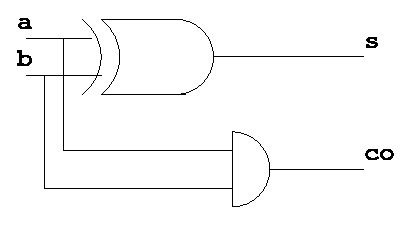
\includegraphics[width=0.19\textwidth]{Fig/half_adder}
%END IMAGE
%HEVEA\imageflush
\hfil
%BEGIN IMAGE
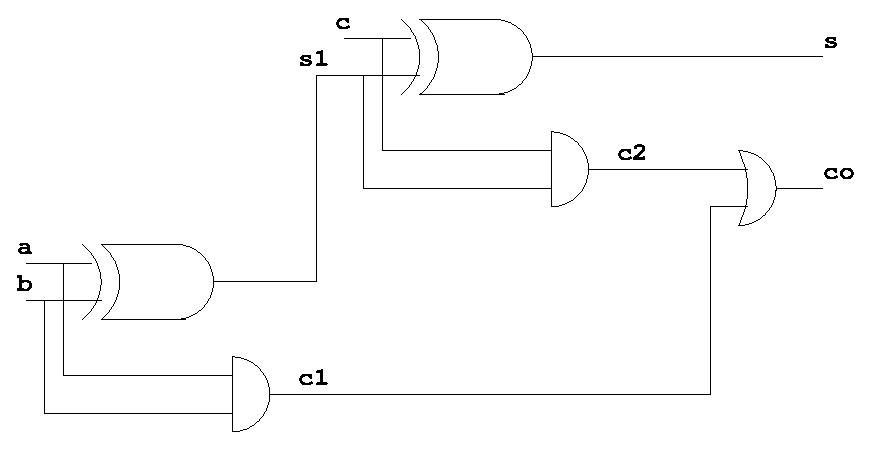
\includegraphics[width=0.4\textwidth]{Fig/full_adder}
%END IMAGE
%HEVEA\imageflush
\caption{A half-adder and a full-adder~\label{half-adder}}
\end{figure}

Alternatively, a full adder can be described more efficiently as a composition
of two half adders. A graphical depiction is given in
\cref{half-adder}. The corresponding program text is:
\begin{runverbatim}[continue,withresult]
let half_add(a,b) = (s, co) where
       s = xor (a, b)
   and co = a & b
\end{runverbatim}
%
\begin{runverbatim}[continue,withresult]
let full_add2(a, b, c) = (s, co) where
  rec (s1, c1) = half_add(a, b)
  and (s, c2) = half_add(c, s1)
  and co = c1 or c2
\end{runverbatim}

The \zls{rec} keyword specifies that the block of equations following the 
\zls{where} is defined by mutual recursion.
Without it the \zls{s1} in the equation for \zls{s} and \zls{c2} would have 
to exist in the list of inputs or the global environment, and similarly for 
\zls{c1} and \zls{c2} in the equation for \zls{co}.

\paragraph{Alternative notation:} For combinatorial function definitions, 
the keyword \zls{let} can be replaced by \zls{fun}.
\begin{runverbatim}[include=xor]
fun half_add (a,b) = (s, co) where
  rec s = xor (a, b)
  and co = a & b
\end{runverbatim}

% }-}3
\subsection{Stateful Functions}\label{sec:sequential-functions} %{-{3

A function is stateful or \emph{sequential} if its output at an instant~$n$ 
depends on the inputs at previous instants~$k$ ($k \leq n$), that is, on the 
history of inputs.
Such functions may produce a varying output signal even when their inputs 
are constant.
%Stateful or \emph{sequential} functions are
%such that their output
%at some instant $n$ may depend on the history of their inputs, that is,
%input values of instants $k$ ($k \leq n$).
%A function is called
%sequential if it may produce a non constant output signal even when its
%inputs are constant. Otherwise, we call it combinatorial.
%A
%sufficient condition to be a combinatorial expression is not to
%contain any delay, initialization operator, nor automaton.

Stateful functions must be declared with the \zls{node} keyword.
For example, this function computes the sequence of integers starting at an 
initial value given by the parameter \zls{m}:
\begin{runverbatim}[withresult]
let node from m = nat where
  rec nat = m -> pre nat + 1
\end{runverbatim}

\noindent
The type signature \zlsmsg{int -D-> int} indicates that \zls{from} is
a sequential function that maps one integer stream to another.
The \zls{D} indicates that this function is stateful, it stands for 
``discrete''.
The functions output may depend on the past values of its input.

Applying this function to the constant stream \zls{0} yields the
execution:
\begin{chrono}{l|ccccccc}
\hline
\zls{m}                 & 0    & 0 & 0 & 0 & 0 & 0 & $\cdots$ \\ \hline
\zls{1}                 & 1    & 1 & 1 & 1 & 1 & 1 & $\cdots$ \\ \hline
\zls{pre nat}           & \nil & 0 & 1 & 2 & 3 & 4 & $\cdots$ \\ \hline
\zls{pre nat + 1}       & \nil & 1 & 2 & 3 & 4 & 5 & $\cdots$ \\ \hline
\zls{m -> pre nat + 1}  & 0    & 1 & 2 & 3 & 4 & 5 & $\cdots$ \\ \hline
\zls{from m}            & 0    & 1 & 2 & 3 & 4 & 5 & $\cdots$ \\ \hline
\end{chrono}

The fact that a function is combinatorial is verified during compilation.
Thus, omitting the \zls{node} keyword,
\begin{runverbatim}[fail]
let from n = nat where rec nat = n -> pre nat + 1
\end{runverbatim}
leads to an error message:
\begin{sample}\runverbatimcmd\end{sample}
\runverbatimerr{}
While a node (arrow type \zlsmsg{-D->}) cannot be called within a 
combinatorial function, it is possible to call a combinatorial function
(arrow type \zlsmsg{-A->}) within in a
node. For example, the addition operator in the \zls{from} function has the 
type signature \zlsmsg{int * int -A-> int}.

\medskip\noindent
The edge front detector is defined a global function from boolean streams to
boolean streams:%
\begin{runverbatim}[withresult]
let node edge c = c & not (false fby c)
\end{runverbatim}
\begin{chrono}{l|ccccccc}
\hline
\zls{c}                 & \f & \f & \t & \t & \f &  \t & $\cdots$ \\ \hline
\zls{false}             & \f & \f & \f & \f & \f &  \f & $\cdots$ \\ \hline
\zls{false fby c}       & \f & \f & \f & \t & \t &  \f & $\cdots$ \\ \hline
\zls{not (false fby c)} & \t & \t & \t & \f & \f &  \t & $\cdots$ \\ \hline
\zls{edge c}            & \f & \f & \t & \f & \f &  \t & $\cdots$ \\ \hline
\end{chrono}

\medskip\noindent
A forward Euler integrator is defined by:
\begin{runverbatim}[withresult,label=integr]
let dt = 0.01
let node integr (x0, x') = x where
  rec x = x0 -> pre (x +. x' *. dt)
\end{runverbatim}
These declarations give a global function \zls{integr} that returns a stream 
\zls{x} defined
recursively so that, for all $n \in \Nat, x(n) = x0 + \sum_{i=0}^{n-1}
x'(i)\cdot dt$.  The operators `\zls{+.}', `\zls{*.}' are, respectively, 
addition and multiplication over floating-point numbers. Sequential
functions are composed just like any other function, as, for example, in:
\begin{runverbatim}[continue]
let node double_integr (x0, x0', x'') = x where
  rec x = integr (x0, x')
  and x' = integr (x0', x'')
\end{runverbatim}

\paragraph{Alternative notation:}
The keyword \zls{let} can be omitted, for example,
\begin{runverbatim}[skipone]
let dt = 0.01
node integr (x0, x') = x where
  rec x = x0 -> pre (x +. x' *. dt)
\end{runverbatim}


% \subsection{Anonymous Functions}
% Functions can be defined in an anonymous way and can be used as
% values. Anonymous combinatorial functions are introduced using a
% single arrow ({\tt ->}), anonymous sequential ones using a double
% arrow ({\tt =>}). For example, the expression \verb#fun x y -> x + y#
% is the sum function and has type \verb#int -> int -> int#). The
% expression \verb#fun x y => x fby x fby y# defines a double delay and
% has the type \verb#'a -> 'a => 'a#.

% The functions \verb-average- and \verb-from- can be defined as:
% \begin{runverbatim}
% let average = fun (x,y) -> (x + y) / 2
% let from = fun n => nat where rec nat = n -> pre nat + 1
% \end{runverbatim}

% }-}3
\subsection{Local and Mutually Recursive Definitions} %{-{3
\label{sec:local-defin-mutu}

Variables may be defined locally with \zls{let}/\zls{in} or
\zls{let rec}/\zls{in} whether the defining expression is stateful or not.
The following
program computes the Euclidean distance between two points:%
\begin{runverbatim}
let distance ((x0,y0), (x1,y1)) =
  let d0 = x1 -. x0 in
  let d1 = y1 -. x1 in
  sqrt (d0 *. d0 +. d1 *. d1)
\end{runverbatim}
Since \zls{d0} and \zls{d1} denote infinite streams, the computations of 
\verb+x1 -. x0+ and \verb+y1 -. x1+ occur in parallel, at least 
conceptually.
In Zélus, however, the consecutive nesting of \zls{let}/\zls{in}s introduces 
a sequential ordering on the computations at an instant.
In this example, this means that the current value of \zls{d0} is always 
computed before the current value of \zls{d1}.
Being able to impose such an ordering is useful when functions with 
side-effects are imported from the host language.
Write simply \zls{let rec d0 = ... and d1 = ...} if no particular ordering 
is needed.

Streams may be defined through sets of mutually recursive equations.  The
function that computes the minimum and maximum of an input stream
\zls{x} can be written in at least three equivalent ways.
As two mutually recursive equations after a \zls{where}:
\begin{runverbatim}
let node min_max x = (min, max) where
  rec min = x -> if x < pre min then x else pre min
  and max = x -> if x > pre max then x else pre max
\end{runverbatim}
as a stream of tuples defined by two local, mutually recursive equations:
\begin{runverbatim}
let node min_max x =
  let rec min = x -> if x < pre min then x else pre min
  and max = x -> if x > pre max then x else pre max in
  (min, max)
\end{runverbatim}
or as a stream of tuples defined by a single recursive equation:
\begin{runverbatim}
let node min_max x = (min, max) where
  rec (min, max) = (x, x) -> if x < pre min then (x, pre max)
                             else if x > pre max then (pre min, x)
                             else (pre min, pre max)
\end{runverbatim}

\noindent Discrete approximations to the sine and cosine functions can be 
defined by:
\begin{runverbatim}[continue,include=integr]
let node sin_cos theta = (sin, cos) where
  rec sin = integr(0.0, theta *. cos)
  and cos = integr(1.0, -. theta *. sin)
\end{runverbatim}

% }-}3
\subsection{Shared Memory and Initialization} %{-{3

In addition to the delay operator \zls{pre}, Zélus provides another 
construction for referring to the previous value of a stream: \zls{last o}, 
where \zls{o} is a variable defined by an equation. For example:%
\begin{runverbatim}
let node counter i = o where
  rec init o = i
  and o = last o + 1
\end{runverbatim}
The equation \zls{init o = i} defines the initial value of the \emph{memory} 
\zls{last o}. This memory is initialized with the first
value of \verb-i-, and thereafter it contains the previous value of
\verb-o-. The above program is thus equivalent to the following
one:\footnote{The construction \texttt{last} is eliminated during 
compilation by a similar transformation.}
\begin{runverbatim}
let node counter i = o where
  rec last_o = i -> pre o
  and o = last_o + 1
\end{runverbatim}
The reason for introducing memories, will become clear when control 
structures are introduced in \cref{sec:patternmatch}.
Syntactically, \verb-last- is {\em not} an operator: \verb-last o- denotes
a shared memory and the argument of \verb-last-, here \verb-o-, must be a 
variable name. Thus this program is rejected:
\begin{runverbatim}[fail,withresult]
let node f () = o where
  rec o = 0 -> last (o + 1)
\end{runverbatim}

Rather than define the current value of a signal in terms of its previous
one, the next value can also be defined in terms of the current one.
The same counter program can be written:
\begin{runverbatim}
let node counter i = o where
  rec init o = i
  and next o = o + 1
\end{runverbatim}
or equivalently:
\begin{runverbatim}
let node counter i = o where
  rec next o = o + 1 init i
\end{runverbatim}
In both definitions, \texttt{o} is initialized with the first value of
\verb-i- and then the value of \texttt{o} at instant $n+1$ is the value of
\verb-o + 1- at instant $n$ (for all $n \in \Nat$).

Neither the form defining the current value from the previous one, nor the 
form defining the next value from the current one is intrinsically superior; 
it depends on the situation.
Either form can be transformed into the other.
We will see in \cref{chap:ode-programming} that restrictions apply to both 
the \verb-next- and \verb-last- constructions when combining discrete- and
continuous-time dynamics.

\Remark The compiler rewrites \verb-last-, \verb+->+, \verb-fby-, 
\verb+pre+, \verb+init+ and \verb+next+ into a minimal subset.

% }-}3
\subsection{Causality check}\label{causality-check} %{-{3

Instantaneous cycles between recursively defined values---\emph{causality 
loops}---are forbidden so that the compiler can produce statically-scheduled 
sequential code.
For example, the program:%
\begin{runverbatim}[fail]
let node from m = nat where
  rec nat = m -> nat + 1
\end{runverbatim}
is rejected with the message:
\runverbatimerr{}
\noindent
This program cannot be computed since \verb+nat+ depends instantaneously on 
itself.
The compiler statically reject function definitions which cannot be 
scheduled sequentially, that is streams whose value at instant $n$ may 
depend on some value at instant $n$.
In practice, it imposes that any loop
crosses a delay \verb-pre- or \verb-fby-. The purpose of
the \emph{causality analysis} to to reject those loops.

\newcommand{\temp}{\mathit{temp}}

Note that delays can be hidden internally in the body of a function as
this is the case for the languages \lustre{} and \signal, for
example. E.g., consider the initial value problem:
\[
\dot{\temp} = g_0 - g_1 \cdot \temp \quad \temp(0) = t_0
\]
Approximate the integration with the explicit Euler integrator defined previously. The
signal $\temp$ can be implemented by the following recursive equation.
\begin{runverbatim}[withresult,include=integr]
(* [t0] is the initial temperature; [g0] and [g1] two constant *)
let node heater(t0, g0, g1) = temp where
  rec temp = integr(t0, g0 -. g1 *. temp)
\end{runverbatim}
This feedback loop is accepted because \verb+integr(t0, g0 -. g1 *. temp)+ does
not depend instantaneously on its input.

It is also possible to force a function to be considered to be strict
by adding the keyword \texttt{atomic}. E.g., the following program is
now rejected by the causality analysis.
%
\begin{runverbatim}[fail,withresult]
let atomic node f x = 0 -> pre (x + 1)
let node wrong () =
  let rec o = f o in o
\end{runverbatim}
%
Indeed, whereas the output of \texttt{f} does not instantaneously
depend on its input \texttt{x}, adding the keyword \texttt{atomic}
forces to consider that all output instantaneously depend on all
inputs. For atomic functions, the compiler produces a single step
function which is simply called.\footnote{Modular code generation
  where a function is split into a minimal set of functions, as
  proposed in~\cite{lucy:emsoft09,lustre:tripakis-popl09}, is not
  implemented in the current version of the compiler. Some functions
  are inlined, according to the dependence information
  computed by the causality analysis.}

%}-}3
\subsection{Initialization check} %{-{3
\label{initialisation-check}
The compiler checks that every delay operator is initialized. For
example:
\begin{runverbatim}[fail,withresult]
let node from m = nat where
  rec nat = pre nat + 1
\end{runverbatim}
The analysis is a {\em one-bit} analysis where expressions are
considered to be either always defined or always defined except at the
very first instant.  It is defined in~\cite{lucy:sttt04}. In
practice, it rejects expressions like \verb-pre (pre e)-, that is,
un-initialized expressions cannot be used as an argument of a delay
and must be first initialized using \verb+->+.

% }-}3
% }-}2
\section{Data-types, Pattern matching} %{-{2

\subsection{Type definitions} %{-{3
Product types, record types and enumerated type may be defined with a
notation close to that of \ocaml. Nonetheless, no constructors with
arguments are allowed for the moment. It is nonetheless possible to
define abstract types and to inport functions from an \ocaml{} module.
See the present reference manual for syntactic considerations.

Records are defined as in Ocaml and accessed with the dot notation. E.g.,
the following defines a type {\tt
  circle}, representing a circle as a record containing a {\tt
  center}, given by its coordinates, and a {\tt radius}.
\begin{runverbatim}
type circle = { center: float * float; radius: float }

let center c = c.center
let radius c = c.radius
\end{runverbatim}
  
% }-}3
\subsection{Pattern matching}\label{sec:patternmatch} %{-{3

The language provides means for doing pattern matching over streams
with a \verb-match/with- construction {\em \`a la} \ocaml.

Consider the example of a colored wheel rotating on an axis and for
which we want to compute the rotation direction. This wheel is
composed of three sections with colors blue (\verb-Blue-), red
(\verb-Red-) and green (\verb-Green-).  A sensor observes the
successive colors on the wheel and has to decide if the wheel is
immobile or determine the rotation direction.

We consider that the direction is direct (\verb-Direct-) when there is
a succession of \verb-Red-, \verb-Green-, \verb-Blue-, \verb-Red-...,
the opposite direction being indirect (\verb-Indirect-). There are
some instants where the direction is undetermined
(\verb-Undetermined-) or that the wheel is immobile (\verb-Immobile-).

We program the controler in the following way. First, we introduce two
sum types.  The function \verb-direction- then compares three
successive values of the input stream \verb-i-.
\begin{runverbatim}
type color = Blue | Red | Green
type dir = Direct | Indirect | Undetermined | Immobile
\end{runverbatim}
%
\begin{runverbatim}[continue,withresult]
let node direction i = d where
  rec pi = i fby i
  and ppi = i fby pi
  and match ppi, pi, i with
  | (Red, Red, Red) | (Blue, Blue, Blue) | (Green, Green, Green) ->
         do d = Immobile done
  | (_, Blue, Red) | (_, Red, Green) | (_, Green, Blue) -> 
         do d = Direct done
  | (_, Red, Blue) | (_, Blue, Green) | (_, Green, Red) -> 
         do d = Indirect done
  | _ -> do d = Undetermined done
  end
\end{runverbatim}

The handler of a pattern-matching construct is made of a set of
equations defining {\em shared} variables (here the variable
\verb-d-). At each instant, the \verb-match/with- statement selects
the first pattern (from top to bottom) which matches the actual value
of the triple \verb-pii, pi, i- and executes the corresponding
branch. During a reaction, only one branch is executed.

Because only one branch is executed during a reaction, one must be
careful when programming with such control structures, in particular
in the presence of delay operators. This can be illustrated on the
following program. This program is made of two modes: in the \verb-Up-
mode, the variable \verb-o- increases by step \verb-1- whereas in the
mode \verb-Down-, it decreases by step \verb+-1+.
\begin{runverbatim}
type modes = Up | Down

let node two (m, i) = o where
  rec init o = i
  and match m with
      | Up -> do o = last o + 1 done
      | Down -> do o = last o - 1 done
      end
\end{runverbatim}
The equation \verb-init o = i- defines a shared memory \verb-last o-
which is initialized with the first value of \verb-i-. \verb-o- is
called a shared variable because it is defined by several
equations. When \verb-m- equals \verb-Up-, \verb-o- equals
\verb-last o + 1-. When \verb-m- equals \verb-Down-, \verb-o- equals
\verb+last o - 1+.  The communication between the two modes is done
through a shared memory \verb-last o-.  \verb-last o- contains the
previous value of \verb-o-, the last time \verb-o- has been
defined. The execution diagram for some execution is given below.
\begin{chrono}{l|cccccccc}
\hline
\tt i                 & \tt 0  & \tt 0  & \tt 0 & \tt 0    & \tt 0  & \tt 0    &  \tt 0  & \dots \\
\hline
\tt m                 & \tt Up & \tt Up & \tt Up & \tt Down & \tt Up & \tt Down &  \tt Down & \dots \\
\hline
\tt last o + 1        & \tt 1  & \tt 2  & \tt 3  &          & \tt 3  &       & 
& \dots \\
\hline
\tt last o - 1        &        &        &        & \tt 2    &        & \tt 2 &  \tt 1   & \dots \\
\hline
\tt o                 & \tt 1  & \tt 2  & \tt 3    & \tt 2    & \tt 3  & \tt 2    &  \tt 1  & \dots \\
\hline
\tt last o            & \tt 0  & \tt 1  & \tt 2    & \tt 3  & \tt 2    &  \tt 3  & \tt 2 & \dots \\
\hline
\end{chrono}

\medskip\noindent
The function \texttt{two} is equivalent to the following one:
\begin{runverbatim}[hide,label=updownmodes]
type modes = Up | Down
\end{runverbatim}
\begin{runverbatim}[continue]
let node two (m, i) = o where
  rec last_o = i -> pre o
  and match m with
      | Up -> do o = last_o + 1 done
      | Down -> do o = last_o - 1 done
      end
\end{runverbatim}
making clear that \verb-last o- stands for the previous defined value
of \verb-o-.

% }-}3
\subsection{Pre versus Last} %{-{3
Whereas \verb-last o- may seem
to be just another way to refer to the previous value of a stream like
\verb-pre o- does, there is a fundamental difference between the
two. This difference is a matter or instant of observation.

\begin{itemize}
\item
In block-diagram formalism {\em \`a la}
\simulink\ or \scade, $\texttt{pre}\;e$ is a unit delay which
is a local memory. $\texttt{pre}$ denotes the last value of its argument, the
last time it was {\em observed}. If $\texttt{pre}\;e$ appears in a
block structure which is executed from time to time --- say when some condition
$c$ is true --- it means that the argument $e$ is only computed when
$c$ is true. Thus $\texttt{pre}\;e$ is the value $e$ had the last time $c$ was true.
\item
$\texttt{last}\;o$ denotes the previous value of the variable $o$ on
  the instant where the variable $o$ is {\em defined}.
  $\texttt{last}\;o$ is syntactically valid when $o$ is a variable name and
  not an expression.  $\texttt{last}\;o$ is useful to communicate
  values between modes and this is why it is called a shared memory.
\end{itemize}

We illustrate the difference between the two on the following
example. We add extra equations on the previous example. The two other streams
\verb-c1- and \verb-c2-
return respectively the number of instants each mode is active.
\begin{runverbatim}[include=updownmodes]
let node two (m, i) = (o, c1, c2) where
  rec init o = i
  and init c1 = 0
  and init c2 = 0
  and match m with
       | Up -> do o = last o + 1
              and c1 = 1 -> pre c1 + 1
              done
       | Down -> do o = last o - 1
                 and c2 = 1 -> pre c2 + 1
                 done
    end
\end{runverbatim}

The equation \verb#c1 = 1 -> pre c1 + 1# is only active in the
\verb-Up- mode whereas equation \texttt{c2 = 1 -> pre c2 + 1} is
active in mode \verb-Down-. The execution diagram is given below.
\begin{chrono}{l|cccccccc}
\hline
\tt i                 & \tt 0  & \tt 0  & \tt 0 & \tt 0    & \tt 0  & \tt 0    &  \tt 0  & \dots \\
\hline
\tt m                 & \tt Up & \tt Up & \tt Up & \tt Down & \tt Up & \tt Down &  \tt Down & \dots \\
\hline
\tt last o + 1        & \tt 1  & \tt 2  & \tt 3  &          & \tt 3  &       & 
& \dots \\
\hline
\tt 1 -> pre c1 + 1   & \tt 1  & \tt 2  & \tt 3  &          & \tt 4  &       & 
& \dots \\
\hline
\tt last o - 1        &        &        &        & \tt 2    &        & \tt 2 &  \tt 1   & \dots \\
\hline
\tt 1 -> pre c2 + 1   &        &        &        & \tt 1    &        & \tt 2 &  \tt 3   & \dots \\
\hline
\tt o                 & \tt 1  & \tt 2  & \tt 3    & \tt 2    & \tt 3  & \tt 2    &  \tt 1  & \dots \\
\hline
\tt last o            & \tt 0  & \tt 1  & \tt 2    & \tt 3  & \tt 2    &  \tt 3  & \tt 2 & \dots \\
\hline
\tt c1                 & \tt 1  & \tt 2  & \tt 3    & \tt 3    & \tt 4  & \tt 4    &  \tt 4  & \dots \\
\hline
\tt c2                 & \tt 0  & \tt 0  & \tt 0    & \tt 1    & \tt 1  & \tt 2    &  \tt 3  & \dots \\
\hline
\end{chrono}

A pattern matching composes several complementary sub-streams.
The above pattern matching has
two branches. Every branch defines its own clock, one denoting the
instants where \verb-m = Up- and the other denoting the instant where
\verb-m = Down-.

% }-}3
\subsection{Local Definitions} %{-{3

It is possible to define variables which stay local to a branch. For
example:
\begin{runverbatim}[include=updownmodes]
let node two (m, i) = o where
  match m with
  | Up -> let rec c = 0 -> pre c + 1 in
          do o = c done
  | Down -> do o = 0 done
  end
\end{runverbatim}
or equivalently:
\begin{runverbatim}[include=updownmodes]
let node two (m, i) = o where
  match m with
  | Up -> local c in
          do c = 0 -> pre c + 1 and o = c done
  | Down -> do o = 0 done
  end
\end{runverbatim}
In the first handler of the \texttt{match/with} statement, \texttt{c} is
declared to be local to the handler. The compiler checks that a definition for
\texttt{c} is given. Several variables can be declared local by writing
\texttt{local c1,..., cn in ...}.

% }-}3
\subsection{Implicit Completion of Shared Variables} %{-{3
Finally, note that the branches of a pattern-matching constraint do
not have to contain a definition for all the shared variables. A
shared variable is implicitly completed as if one has written
equations of the form \verb-x = last x- in branches where no
definition for \verb-x- is given. Finally, the compiler rejects situations
where it is unable to ensure that an initial value exist for
\texttt{last x}. Thus, the following program is rejected.
\begin{runverbatim}[withresult,fail,include=updownmodes]
let node two (m, i) = o where
  rec match m with
      | Up -> do o = last o + 1 done
      | Down -> do o = last o - 1 done
      end
\end{runverbatim}

% \begin{verbatim}
% type event = Click | Move | Keypressed of char

% (* count the number of Move between two click *)
% let node count e = cpt where
%   rec last o = 0
%   and match e with
%         Top -> do o = last o + 1 done
%       | Click -> do o = last o done
%       end
% \end{verbatim}

% A pattern matching composes several complementary sub-streams, that
% is, streams on complementary clocks. The above pattern matching 
% has two branches. Every branch defines its own clock, one denoting
% the instants where \verb-e = Top- and the other denoting the instant
% where \verb-e = Click-.

% The branch \verb#Top when clk -> (pre o) when clk + 1#
% states that for the instants where the condition \verb-e = Top- is
% true (\verb-clk- being the clock of this branch), the result is the
% previous value of \verb-o- plus one. For the instants where
% \verb-e = Click-, the result is \verb-0-.

% The pattern-matching construction is very similar to the \verb-merge-
% construction and thus, benefit (and somethimes suffers ?) from the same clock
% constraints. Thus, writing simply \verb-(pre o) + 1- would lead to a
% clocking error since \verb-o- is on the base clock and must be sampled
% on the clock of the branch.

% The execution diagram is given below.

% \vspace{.5cm}

% \begin{tabular}
% {c|ccccccc}
% \hline
% \tt e                 & \tt Click & \tt Top & \tt Top & \tt Click & \tt Top &  \tt Click & \dots \\
% \hline
% \tt clk		      & $f$   & $t$ & $t$ & $f$   & $t$ &  $f$ & \dots \\
% \hline
% \tt Top when clk      &       & \tt Top & \tt Top &       & \tt Top &      & \dots \\
% \hline
% \tt (pre o) when clk + 1
%                       &       & $1$ & $2$ &       & $1$ &      & \dots \\
% \hline
% \tt Click             & \tt Click   &   &  & \tt Click   &   &  \tt Click & \dots \\
% \hline
% \tt 0                 & $0$   &  &  & $0$   &  &  $0$ & \dots \\
% \hline
% \tt o                 & $0$   & $1$ & $2$ & $0$   & $1$ &  $0$ & \dots \\
% \hline
% \end{tabular}

% \vspace{.5cm}

% This program can also be written in the following way:
% \begin{verbatim}
% let count e =
%   let rec o =
%     0 -> match e, pre o with
%       Top, o -> o + 1
%     | _ -> 0 in
%   o
% \end{verbatim}

% If we get back to the first version of the \verb-count- function, the reader may
%  notice the difference between an expression
% \verb-(pre o) when clk- which refers to ``the value of \verb-o- at the last
% global instant'' and \verb-pre (o when clk)- which refers ``the value
% of \verb-o- at the last instant where \verb-clk- was true''. To illustrate
% this difference, consider now the problem of counting the distance
% made by a mouse between two clicks.

% \begin{verbatim}
% (* computes the distance between two click *)
% let distance pos_x e =
%   0 -> match e with
%     Click when c -> pos_x when c - pre (pos_x when c)
%   | Top -> 0

% (* second way *)
% let distance d e =
%   0 -> match e, d with
%     Click, d -> d - pre d
%   | _ -> 0
% \end{verbatim}
% The execution diagram is given below.

% \vspace{.5cm}

% \begin{tabular}
% {c|ccccccc}
% \hline
% \tt pos\_x                 & $1$       & $2$     & $3$     & $3$       & $3$ &  $5$ & \dots \\
% \hline
% \tt e                 & \tt Click & \tt Top & \tt Top & \tt Click & \tt Top &  \tt Click & \dots \\
% \hline
% \tt Click when c      & \tt Click   &  & & \tt Click      & &  \tt Click  & \dots \\
% \hline
% \tt pos\_x when c     & $1$       &     &     & $3$       &  &  $5$ & \dots \\
% \hline
% \tt pre (pos\_x when c) & $nil$   &     &     & $1$       &  &  $3$ & \dots \\
% \hline
% \tt pos\_x when c -
% pre (pos\_x when c)      & $nil$  &     &     & $2$       &  &  $2$ & \dots \\
% \hline
% \tt distance d e       & $0$       & $0$&     & $2$        & $0$ & $2$ & \dots \\
% \hline
% \end{tabular}

% \vspace{.5cm}
% The \verb-match/with- construction is a generalised form of
% \verb-merge-. These constructions are the natural way to express
% control structure in a data-flow language. In the example above, the
% computation  
% \verb+pos_x when c - pre (pos_x when c)+ is only executed when
% \verb-e- equals \verb-Click-. The compilers deeply rely on clocks for
% generating good imperative code.

\section{Valued Signals}
\label{signals}
The language provides a way to manage {\em valued signals}. Signals
are built and accessed through the constructions \verb-emit- and
\verb-present-.  At every instant, a value signal is a pair made of (1) a boolean
$c$ indicating when the signal is present and (2) a value present when $c$ is
true.\footnote{For \ocaml{} programmers, a signals correspond to a value
of an option type.}
 
% }-}3
\subsection{Signal Emission} %{-{3

It is also possible to define the value of a signal at certain instant only,
that is, not to implictly keep the previous value as we illustrated with
shared variables. % As opposed to shared variables, it is now possible to give a
% partial definition with no implicit completion.
Consider the following program:
\begin{runverbatim}[withresult]
let node within (min, max, x) = o where
  rec c = (min <= x) & (x <= max)
  and present c -> do emit o = () done
\end{runverbatim}
It computes a condition \verb-c-. Then \verb-o- is a signal
which is present with value \verb-()- every time \verb-c- is
true. There is no need here to give an initial value to \verb-o-. When \verb-c- is
false, \verb-o- is simply absent. Writting the following program would lead to
an error:
\begin{runverbatim}[withresult,fail]
let node within (min, max, x) = o where
  rec c = (min <= x) & (x <= max)
  and present c -> do o = () done
\end{runverbatim}

% }-}3
\subsection{Testing the Presence of a Signal and Accessing its Value} %{-{3
It is possible to test for the presence of a signal expression $e$ by
writing the boolean expression $? e$. The following program, for
example, counts the number of instants where \verb-x- is emitted.
\begin{runverbatim}[withresult]
let node count x = cpt where
  rec cpt = if ?x then 1 -> pre cpt + 1 else 0 -> pre cpt
\end{runverbatim}

The language provides a more general mechanism to test for the
presence of several signals and access their values. It is reminiscent
of the pattern-matching construct of ML.  This pattern matching
mechanisn is safe in the sense that it is possible to access the value
of a signal only at the instant where it is emitted.\footnote{This
  contrasts the \esterel{} solution where the value of a signal
  implicitly holds and can be accessed even when it is not
  emitted. The constraint imposed by \zelus{} may be cumbersome in some circumstances,
  but it is safer. It avoids initialization issues and
  the need to allocate a state variable to store the previous
  value.}

The following program takes two signals \verb-x- and \verb-y- and
returns an integer which equals the sum of \verb-x- and \verb-y- when
both are emitted, it returns the value of \verb-x- when \verb-x- is
emitted only and the value \verb-0- when only \verb-y- is emitted and
\verb-0- otherwise.
\begin{runverbatim}[withresult]
let node sum (x, y) = o where
  present
  | x(v) & y(w) -> do o = v + w done
  | x(v1) -> do o = v1 done
  | y(v2) -> do o = v2 done
  else do o = 0 done
  end
\end{runverbatim}
A \verb-present- statement is made of several signal conditions and
handlers. Each condition is tested sequentially. The signal condition
\verb-x(v) & y(w)- is verified when both signals \verb-x- and \verb-y-
are present. A condition \verb-x(v1)- means ``\verb-x- is present and
has some value \verb-v1-''. The variable \verb-v1- can in turn be used
in the corresponding handler.

In the signal pattern \verb-x(v) & y(w)-, \verb-x- and \verb-y- are
expressions evaluating to signal values whereas \verb-v- and \verb-w-
stand for patterns. Thus, writing \verb-x(42) & y(w)- would mean:
``await for the presence of signal \verb-x- evaluating to \verb-42-
and the presence of \verb-y-.

Note that the output of the function \verb-sum- is a regular flow
since the test is exhaustive. Forgetting the default case will raise
an error.
\begin{runverbatim}[withresult,fail]
let node sum (x, y) = o where
  present
  | x(v) & y(w) -> do o = v + w done
  | x(v1) -> do o = v1 done
  | y(v2) -> do o = v2 done
  end
\end{runverbatim}

We can easily eliminate this error by giving a last value to \verb-o-
(e.g., adding an equation \verb-init o = 0- outside of the present
statement). In that case, the default case is implicitly completed
with an equation \verb-o = last o-. The other way is to state that
\verb-o- is now a signal and is thus only partially defined.
\begin{runverbatim}[withresult]
let node sum (x, y) = o where
  present
  | x(v) & y(w) -> do emit o = v + w done
  | x(v1) -> do emit o = v1 done
  | y(v2) -> do emit o = v2 done
  end
\end{runverbatim}

A signal pattern may also contain boolean expressions. The following
program, sums the values of the two signals \verb-x- and \verb-y-
provided they arrive at the same time and \verb-z >= 0-.
\begin{runverbatim}
let node sum (x, y, z) = o where
  present
    x(v) & y(w) & (z >= 0) -> do o = v + w done
  else do o = 0 done
  end
\end{runverbatim}

\Remark Using signals, it is possible
to mimic the
\verb-default- construction of the language
\signal~\cite{signal:scp91}. \verb-default x y- emits the value of \verb-x- when \verb-x-
is present and the value of \verb-y- when \verb-x- is absent and
\verb-y- is present. The signal pattern \verb+x(v) | y(v)+ tests the
presence of ``\verb-x- or \verb-y-''.
\begin{runverbatim}
let node default (x, y) = o where
  present
    x(v) | y(v) -> do emit o = v done
  end
\end{runverbatim}
This is only a simulation since all the information about the precise
instants where \verb-x- and \verb-y- are present --- the so-called
\emph{clock calculus} of \signal~\cite{signal:scp91} --- are hidden at
run-time and not exploited by the compiler. In particular, the
compiler is unable to state that \verb-o- is emitted only when
\verb-x- or \verb-y- are present as the clock calculus of
\signal{} does for the default operator.

The current version of \zelus{} does not provide a \emph{clock calculus} as
\lustre, \lucy{} and \signal{} did.

\section{Hierarchical State Machines}
The language provides means to define hierachical state
machines. These state machines can be composed in parallel with
regular equations or other state machines and can be arbitrarily
nested. State machines are essentially borrowed \emph{as is} from \lucy{} 
and 
\footnoteurl{\scadesix.}{http://www.esterel-technologies.com/products/scade-suite/}
Their compilation is that of~\cite{lucy:emsoft05b}.

In this tutorial, we first consider state machines where transitions
are only made of boolean expressions. Then, we consider two important
extensions of the basic model. The first one is the ability to build
define state machines with parameterized states and actions on
transitions. The second one introduces the general form of transitions
made of signal matching and boolean expressions.

An automaton is a collection of states and transitions. Two kinds of
transitions are provided, namely {\em weak} and {\em strong}
transitions and for each of them, it is possible to enter in the next
state by {\em reset} or by {\em history}. One important feature of
these state machines is that {\em only one set of equations is
  executed during one reaction}.

% }-}3
\subsection{Strong Preemption} %{-{3
Here is a two state automaton illustrating strong preemption. The
function \verb-expect- awaits \verb-x- to be true and emits
\verb-true- for the remaining instants.
\begin{runverbatim}[continue,withresult]
(* await x to be true and then sustain the value *)
let node strong x = o where 
  automaton
  | S1 -> do o = false unless x then S2
  | S2 -> do o = true done
  end
\end{runverbatim}

This automaton is made of two states, each of them defining the value
of a {\em shared} variable \verb-o-. The keyword \verb-unless-
indicates that \verb-o- is defined by the equation \verb-o = false-
from state \verb-S1- while \verb-x- is false. At the instant where
\verb-x- is true, \verb-S2- becomes the active state for the remaining
instant. Thus, the following chronogram hold:
\begin{chrono}{c|ccccccc}
\hline
\tt x                 & \tt false & \tt false & \tt true & \tt false & \tt false &  \tt true & \dots \\
\hline
\tt expect x           & \tt false & \tt false & \tt true & \tt true & \tt true &  \tt true & \dots  \\ \hline
\end{chrono}

% }-}3
\subsection{Weak Preemption} %{-{3

On the contrary, the following function emits \verb-false- at the
instant where \verb-x- is true and \verb-true- for the remaining
instants, thus corresponding to regular {\em Moore automata}.
\begin{runverbatim}[label=expect,withresult]
(* await x to be true and then sustain the value *)
let node expect x = o where 
  automaton
  | S1 -> do o = false until x then S2
  | S2 -> do o = true done
  end
\end{runverbatim}

\begin{chrono}{c|ccccccc}
\hline
\tt x                 & \tt false & \tt false & \tt true & \tt false & \tt false &  \tt true & \dots \\
\hline
\tt expect x           & \tt false & \tt false & \tt false & \tt true & \tt true &  \tt true & \dots  \\ \hline
\end{chrono}

The classical two states \verb-switch- automaton can be written like
the following:
\begin{runverbatim}
let node weak_switch on_off = o where
  automaton
  | False -> do o = false until on_off then True
  | True -> do o = true until on_off then False
  end
\end{runverbatim}

Note the difference with the following form with weak transitions only:
\begin{runverbatim}[continue]
let node strong_switch on_off = o where
  automaton
  | False -> do o = false unless on_off then True
  | True -> do o = true unless on_off then False
  end
\end{runverbatim}

We can check that for any boolean stream \verb-on_off-, the following
property holds:
\begin{runverbatim}[continue,skipone]
let node correct on_off =
weak_switch on_off = strong_switch (false -> pre on_off)
\end{runverbatim}
The graphical representation of these two automata is given in
figure~\cref{switch-figure}.

\begin{figure}
%BEGIN IMAGE
\begin{center}
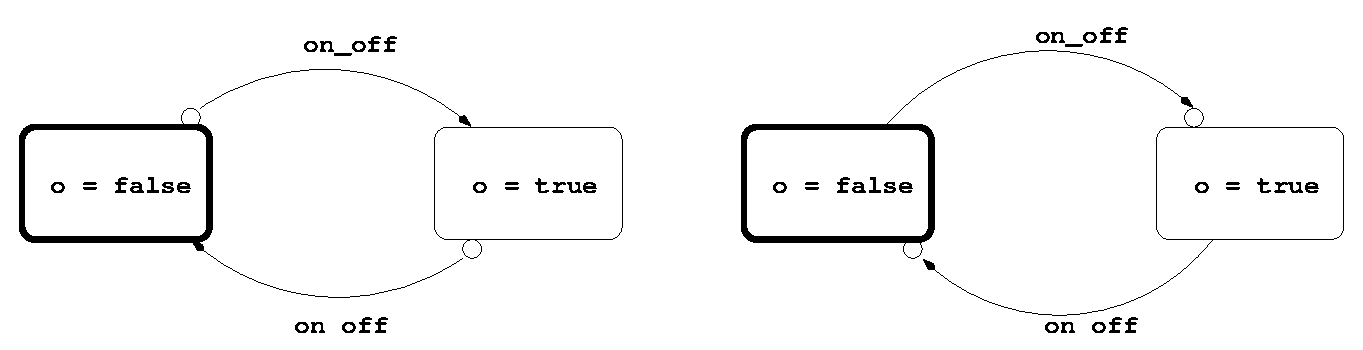
\includegraphics[width=\textwidth]{Fig/automaton}
\end{center}
%END IMAGE
%HEVEA\imageflush
\caption{Two automata with strong and weak transitions~\label{switch-figure}}
\end{figure}

% Weak and strong conditions can be arbitrarily mixed as in the
% following variation of the switch automaton:
% \begin{runverbatim}
% let node switch2 (on_off, stop) = o where
%   automaton
%   | False -> do o = false until on_off then True
%   | True -> do o = true until on_off then False unless stop then Stop
%   | Stop -> do o = true done
%   end
% \end{runverbatim}
%
%Compared to the previous version, state \verb-True- can be strongly
%preempted when some stop condition \verb-stop- is true.

% }-}3
\subsection{Parameterized State Machines} %{-{3
In the examples we have considered so far, an automaton is made of a
finite set of states and transitions. It is possible to define more
general state machines containing parameterized states, that is,
states that may be initialized with some input values. Parameterized
states are a natural way to pass informations from states to states
and to reduce the number of states. Parameterized state machine
lead to a particular style of programming similar to the
definition of mutually tail-recursive functions in ML. Yet they are not
compiled into mutually recursive functions but into a single step
function with a \texttt{switch}-like construct according to the current
active state.

The following function awaits for an event \texttt{e}. When \texttt{e} is present with
a value \texttt{v}, the next state becomes \texttt{Sustain(v)} with the parameter
\texttt{x} of state \texttt{Sustain} set to \texttt{v}.
\begin{runverbatim}[withresult,label=await]
(* await e to be present and sustain its value for the remaining instants *)
let node await e = o where 
  automaton
  | Await -> do unless e(v) then Sustain(v)
  | Sustain(x) -> do emit o = x done
  end
\end{runverbatim}

Note that the formal parameter \verb-x- of state \verb-Sustain- could
be used without restriction in the body of the state. In the same way, the
argument \verb-v- could be replaced by any expression.

\medskip
The following program is a quite radical use of parameterized states: it
is a simple counter that counts the number of
occurrences of \verb-x-.
\begin{runverbatim}[withresult]
let node count x = o where rec o = 0 -> pre o + 1

let node count_in_an_automaton x = o where
  automaton
  | Zero -> do o = 0 until x then Plus(1)
  | Plus(v) -> do o = v until x then Plus(v+1)
  end
\end{runverbatim}

This automaton simulates an infinite state machine with states
\verb-Zero-, \verb-Plus(1)-, \verb-Plus(2)-, etc.

% }-}3
\subsection{ABRO and Modular Reseting} %{-{3

The ABRO example is due to G\'erard Berry~\cite{esterel:primer99}. It
highlight the expressive power of parallel composition and preemption
in Esterel. The specification is the following:

\begin{quote}
Awaits the presence of events \verb-A- and \verb-B- and emit \verb-O-
at the exact instant where both events have been received.  Reset this
behavior every time \verb-R- is received.
\end{quote}
Here is how we write it, replacing capital letters by small
letter~\footnote{As in \ocaml, identifiers starting with a capital
  letter are considered to be constructors and cannot be used for
  variables.}. We make it a little more general, considering that
events are valued.

The following function awaits for an event \texttt{e}. When \texttt{e} is present with
a value \texttt{v}, the next state becomes \texttt{Sustain(v)} with the parameter
\texttt{x} of state \texttt{Sustain} set to \texttt{v}.
\begin{runverbatim}[withresult,include=await,label=abo]
(* emit o and sustain it when a and b has been received *)
let node abo (a, b) = o where
  present (await a)(v1) & (await b)(v2) -> do emit o = v1 + v2 done
\end{runverbatim}
%
\begin{runverbatim}[withresult,continue]
(* here is ABRO: the same except that we reset the behavior *)
(* when r is true *)
let node abro (a, b, r) = o where
  automaton
  | S1 ->
       do present (await a)(v1) & (await b)(v2) -> do emit o = v1 + v2 done
       unless r then S1
  end
\end{runverbatim}

The node \verb-abro- is a one state automaton which {\em resets} the
computation of \verb-abo a b-: every stream in \verb-abo a b- restarts
with its initial value. The language provides a specific
\verb-reset/every- primitive as a shortcut of such a one-state
automaton. We can write:
\begin{runverbatim}[withresult,include=await]
let node abro (a, b, r) = o where
  reset
    present (await a)(v1) & (await b)(v2) -> do emit o = v1 + v2 done
  every r
\end{runverbatim}

The \verb-reset/every- construction combines a set of parallel
equations (separated with an \verb-and-). Note that the reset
operation correspond to strong preemption: the body is reseted at the
instant where the condition is true. The language does not provide a
``weak reset''. Nonetheless, it can be programmed adding a unit delay.
\begin{runverbatim}[withresult,include=abo]
  let node abro (a, b, r) = o where
    reset
      o = abo (a, b)
    every true -> pre r
\end{runverbatim}

% It is also possible to write:

% \begin{verbatim}
% let node abro a b r = o where
%   rec automaton
%         S1 -> do automaton
%                    S1 ->
%                     do o = (except a) & (except b)
%                     until o then S2
%                  | S2 -> do o = true done
%                  end
%               unless r then S1
%       end
% \end{verbatim}

We end with a very common situation of a real-time controller that count
the passage of time and change its running mode according to those counter. This
example enlight the difference between logical time as we have considered up to know
and real-time. Consider a light that
blinks with a specification that says:

\begin{quote}
  Repeat infinitely the following behavior:
  Turn light on for \texttt{n} seconds and off for
  \texttt{m} seconds.
\end{quote}

A way of implementing it is this. The signal \texttt{second} is
represented by a boolean, true at every occurrence of a second, false
otherwise. Moreover, we want this to be reset every time \texttt{res}
is true. We first write a node \texttt{after} such that
\texttt{after(n, t)} returns true when \texttt{t} had \texttt{n} true
values. The node \texttt{blink\_reset} is a two mode automaton
surrended by a reset.
\begin{runverbatim}[withresult,label=after,label=blink_reset]
let node after(n, t) = (cpt >= n) where
  rec tick = if t then 1 else 0
  and ok = cpt >= n
  and cpt = tick -> if pre ok then n else pre cpt + tick

let node blink_reset (r, n, m, t) = x where
 reset
   automaton
   | On  -> do x = true  until (after(n, t)) then Off
   | Off -> do x = false until (after(m, t)) then On
 every r
\end{runverbatim}

\medskip
The type signatures inferred by the compiler are:
\runverbatimmsg{}

Does \texttt{after(n, second)} means \texttt{n} real-time seconds? No, for two reasons.
\begin{enumerate}
\item
  \texttt{second} is a Boolean stream. No hypothesis is made by or
  ensured by the compiler about the
  actual real-time duration between two occurrences of the value
  \emph{true}. It is a matter of the implementation to ensure that
  \texttt{second} is a good approximation of a real second.
\item
  The counting of instants in the expression
  \texttt{after(n, t)} is performed only when the expression is active, that is,
  it returns true when \texttt{n} occurrences of the value \emph{true} has
  been \emph{observed}.
\end{enumerate}
In a discrete-time program as we wrote in this chapter, time is not absolute but
logical and local.
  
% }-}3
\subsection{Local Definitions in a State} %{-{3

It is possible to define names which are local to a state. These names
can only be used inside the body of the state and may be used in weak
conditions only.

The following programs integrates the integer sequence \verb-v- and
emits false until the sum has reached some value \verb-max-. Then, it
emits \verb-true- during \verb-n- instants.
\begin{runverbatim}
let node consume (max, n, v) = status where
  automaton
  | S1 ->
      let rec c = v -> pre c + v in
      do status = false
      until (c = max) then S2
  | S2 ->
      let rec c = 1 -> pre c + v in
      do status = true
      until (c = n) then S1
  end
\end{runverbatim}

State \verb-S1- defines a local variable \verb-c- which can be used to
compute the weak condition \verb-c = max- and this does not introduce
any causality problem. Indeed, weak transitions are only effective
during the next reaction, that is, they define the next state, not the
current one. Moreover, there is no restriction on the kind of
expressions appearing in conditions and they may, in particular, have
some internal state. For example, the previous program can be
rewritten as:
\begin{runverbatim}
let node counting v = cpt where
  rec cpt = v -> pre cpt + v

let node consume (max, n, v) = status where
  automaton
  | S1 ->
       do status = false
       until (counting v = max) then S2
  | S2 ->
       do status = true
       until (counting 1 = n) then S1
  end
\end{runverbatim}
The body of a state is a sequence (possibly empty) of local
definitions (with \verb-let/in-) followed by some definitions of
shared names (with \verb-do/until-). As said previously, weak
conditions may depend on local names and shared names.

Replacing \verb-until- by an \verb-unless- leads to an error. Indeed,
in a strong preemption, the condition is evaluated {\em before} the
equations of the body and thus, cannot depend on them. In a weak
preemption, the condition is evaluated at the end, {\em after} the
definitions of the body have been evaluated. Thus, when writing:
\begin{runverbatim}[fail]
let node consume (max, n, v) = status where
  automaton
  | S1 ->
      let rec c = v -> pre c + v in
      do status = false
      unless (c = max) then S2
  | S2 ->
      let rec c = 1 -> pre c + v in
      do status = true
      unless (c = n) then S1
  end
\end{runverbatim}
The compiler emits the message:
\runverbatimerr{}
%\begin{sample}
%File "tutorial.zls", line 6:
%> unless c = max then S2
%>        ^^^^^^^
%This expression may depend on itself.
%\end{sample}
The variable \verb-c- is not visible in the handler of the \verb-unless-. The
same appears if \verb-c- is declared as a local variable.
\begin{runverbatim}[fail]
let node consume (max, n, v) = status where
  automaton
  | S1 ->
      local c in
      do c = v -> pre c + v and status = false
      unless (c = max) then S2
  | S2 ->
      local c in
      do c = v -> pre c + v and status = true
      unless (c = n) then S1
  end
\end{runverbatim}
The compiler emits the message:
\runverbatimerr{}

% }-}3
\subsection{Communication between States and Shared Memory} %{-{3

In the previous examples, there is no communication between values
computed in each state. Consider a simple system made of two running
modes as seen previously. In the \verb-Up- mode, the system increases
some value with a fixed step \verb-1- whereas in the \verb-Down- mode,
this value decreased with the same step. Now, the transition from one
mode to the other is described by a two-state automaton whose behavior
depends on the value computed in each mode. This example, due to
Maraninchi \& R\'emond~\cite{Modes-SCP03} can be programmed in the
following way.
\begin{runverbatim}[include=updownmodes]
let node two_states (i, min, max) = o where
  rec automaton
      | Up -> do o = last o + 1
              until (o = max) then Down
      | Down -> do o = last o - 1
                until (o = min) then Up
      end
  and init o = i
\end{runverbatim}
An execution diagram is given below:
\begin{chrono}
{l|ccccccccccccc}
\hline
\tt i                 & \tt 0  & \tt 0  & \tt 0 & \tt 0    & \tt 0  & \tt 0    &  \tt 0  & \tt 0  & \tt 0 & \tt 0    & \tt 0  & \tt 0   & \dots \\
\hline
\tt min               & \tt 0  & \tt 0  & \tt 0 & \tt 0    & \tt 0  & \tt 0    &  \tt 0  & \tt 0  & \tt 0 & \tt -1    & \tt 0  & \tt 0   & \dots \\
\hline
\tt max               & \tt 4  & \tt 4  & \tt 4 & \tt 4    & \tt 4  & \tt 4    &  \tt 4 & \tt 4  & \tt 4 & \tt 4    & \tt 4  & \tt 4    & \dots \\
\hline
\tt last o            & \tt 0 & \tt 1 & \tt 2 & \tt 3 & \tt 4 & \tt 3 &  \tt 2 
& \tt 1  & \tt 0 & \tt -1    & \tt 0  & \tt 1   & \dots \\
\hline
\tt o            & \tt 1 & \tt 2 & \tt 3 & \tt 4 & \tt 3 & \tt 2 &  \tt 1 
& \tt 0  & \tt -1 & \tt 0    & \tt 1  & \tt 2   & \dots \\
\hline
\tt last o + 1        & \tt 1  & \tt 2  & \tt 3  & \tt 4  &   &   & 
& & & \tt 0 & \tt 1    & \tt 2  & \dots \\
\hline
\tt last o - 1   &    &        &        &        & \tt 3 & \tt 2  & \tt 1
& \tt 0  & \tt -1 &   & & & \dots \\
\hline
\end{chrono}

% }-}3
\subsection{The Particular Role of the Initial State} %{-{3
The initial state can be used for defining some variables whose value
can then be sustained in remaining states. In that case, their last
value is considered to be defined. Moreover, it becomes possible not
to define their value in all the states.
\begin{runverbatim}
let node two_states (i, min, max) = o where
  rec automaton
      | Init ->
           do o = i until (i > 0) then Up
      | Up -> 
          do o = last o + 1
          until (o = max) then Down
      | Down -> 
          do o = last o - 1
          until (o = min) then Up
      end
\end{runverbatim}

\begin{chrono}{l|cccccccccccccccc}
\hline
\tt i                 & \tt 0  & \tt 0  & \tt 0 & \tt 1  & \tt 1  & \tt 1 & \tt 1    & \tt 1  & \tt 1    &  \tt 1  & \tt 1  & \tt 1 & \tt 1    & \tt 1  & \tt 1   & \dots \\
\hline
\tt min               & \tt 0  & \tt 0  & \tt 0  & \tt 0  & \tt 0  & \tt 0 & \tt 0    & \tt 0  & \tt 0    &  \tt 0  & \tt 0  & \tt 0 & \tt -1    & \tt 0  & \tt 0   & \dots \\
\hline
\tt max               & \tt 0  & \tt 0  & \tt 0 & \tt 4  & \tt 4  & \tt 4 & \tt 4    & \tt 4  & \tt 4    &  \tt 4 & \tt 4  & \tt 4 & \tt 4    & \tt 4  & \tt 4    & \dots \\
\hline
\tt last o            & \tt 0  & \tt 0  & \tt 0 & \tt 0 & \tt 1 & \tt 2 & \tt 3 & \tt 4 & \tt 3 &  \tt 2 
& \tt 1  & \tt 0 & \tt -1    & \tt 0  & \tt 1   & \dots \\
\hline
\tt o            & \tt 0  & \tt 0  & \tt 0 & \tt 1 & \tt 2 & \tt 3 & \tt 4 & \tt 3 & \tt 2 &  \tt 1 
& \tt 0  & \tt -1 & \tt 0    & \tt 1  & \tt 2   & \dots \\
\hline
\tt last o + 1     & \tt 0  & \tt 0  & \tt 0    & \tt 1  & \tt 2  & \tt 3  & \tt 4  &   &   & 
& & & \tt 0 & \tt 1    & \tt 2  & \dots \\
\hline
\tt last o - 1   & \tt 0  & \tt 0  & \tt 0 &    &        &        &        & \tt 3 & \tt 2  & \tt 1
& \tt 0  & \tt -1 &   & & & \dots \\
\hline
\end{chrono}

Because the initial state \verb-Init- is only weakly preempted,
\verb-o- is necessarily initialized with the current value of
\verb-i-. Thus, \verb-last o- is well defined in the remaining
states. Note that replacing the weak preemption by a strong one will
lead to an error.
\begin{runverbatim}[fail]
let node two_states (i, min, max) = o where
  rec automaton
      | Init ->
          do o = i unless (i > 0) then Up
      | Up -> 
          do o = last o + 1
          unless (o = max) then Down
      | Down -> 
          do o = last o - 1
          unless (o = min) then Up
      end
\end{runverbatim}
and we get:
\runverbatimerr{}

We said previously that strong conditions must not depend on some
variables computed in the current state but they can depend on some
shared memory \verb-last o- as in:
\begin{runverbatim}[skiptwo]
let node two_states (i, min, max) = o where
rec init o = i
and automaton
      | Init ->
          do o = i unless (i > 0) then Up
      | Up -> 
          do o = last o + 1
          unless (last o = max) then Down
      | Down -> 
          do o = last o - 1
          unless (last o = min) then Up
      end
\end{runverbatim}
and we get the same execution diagram as before:
\begin{chrono}{l|cccccccccccccccc}
\hline
\tt i                 & \tt 0  & \tt 0  & \tt 0 & \tt 1  & \tt 1  & \tt 1 & \tt 1    & \tt 1  & \tt 1    &  \tt 1  & \tt 1  & \tt 1 & \tt 1    & \tt 1  & \tt 1   & \dots \\
\hline
\tt min               & \tt 0  & \tt 0  & \tt 0  & \tt 0  & \tt 0  & \tt 0 & \tt 0    & \tt 0  & \tt 0    &  \tt 0  & \tt 0  & \tt 0 & \tt -1    & \tt 0  & \tt 0   & \dots \\
\hline
\tt max               & \tt 0  & \tt 0  & \tt 0 & \tt 4  & \tt 4  & \tt 4 & \tt 4    & \tt 4  & \tt 4    &  \tt 4 & \tt 4  & \tt 4 & \tt 4    & \tt 4  & \tt 4    & \dots \\
\hline
\tt last o            & \tt 0  & \tt 0  & \tt 0 & \tt 0 & \tt 1 & \tt 2 & \tt 3 & \tt 4 & \tt 3 &  \tt 2 
& \tt 1  & \tt 0 & \tt -1    & \tt 0  & \tt 1   & \dots \\
\hline
\tt o            & \tt 0  & \tt 0  & \tt 0 & \tt 1 & \tt 2 & \tt 3 & \tt 4 & \tt 3 & \tt 2 &  \tt 1 
& \tt 0  & \tt -1 & \tt 0    & \tt 1  & \tt 2   & \dots \\
\hline
\tt last o + 1     & \tt 0  & \tt 0  & \tt 0    & \tt 1  & \tt 2  & \tt 3  & \tt 4  &   &   & 
& & & \tt 0 & \tt 1    & \tt 2  & \dots \\
\hline
\tt last o - 1   & \tt 0  & \tt 0  & \tt 0 &    &        &        &        & \tt 3 & \tt 2  & \tt 1
& \tt 0  & \tt -1 &   & & & \dots \\
\hline
\end{chrono}

% We illustrate the feature on a boucing ball with constant speed
% whose direction only change when some collision occurs.

% \begin{verbatim}
% let node integr x0 dx = x where rec x = x0 -> pre x + dx

% let node bouncing left right x0 dx0 = x where
%   rec automaton
%         Init ->
%           do dx = dx0 then Move
%       | Move -> do until x = left or x = right then Change(-dx)
%       | Change(dir) -> do dx = dir then Move
%       end
%   and x = integr x0 dx
% \end{verbatim}
% We can make a more complicated system where the new direction is the
% result of a computation (e.g., elastic collision with Newton laws).

Note that the escape condition \verb-do x = 0 and y = 0 then Up- in
the initial state is a shortcut for
\verb-do x = 0 and y = 0 until true then Up-.

Finally, \verb-o- do not have to be defined in all the states. In that
case, it keeps its previous value, that is, an equation
\verb-o = last o- is implicitly added.

% }-}3
\subsection{Resume a Local State} %{-{3
By default, when entering in a state, every computation in the state
is reseted. We also provides some means to resume the internal memory
of a state (this is called {\em enter by history} in UML diagrams).
\begin{runverbatim}[include=updownmodes]
let node two_modes (min, max) = o where
  rec automaton
      | Up -> do o = 0 -> last o + 1 until (o >= max) continue Down
      | Down -> do o = last o - 1 until (o <= min) continue Up
      end
\end{runverbatim}

\begin{chrono}{l|cccccccccccccccc}
\hline
\tt min               & \tt 0  & \tt 0  & \tt 0  & \tt 0  & \tt 0  & \tt 0 & \tt 0    & \tt 0  & \tt 0    &  \tt 0  & \tt 0  & \tt 0 & \tt -1    & \tt 0  & \tt 0   & \dots \\
\hline
\tt max               & \tt 0  & \tt 0  & \tt 0 & \tt 4  & \tt 4  & \tt 4 & \tt 4    & \tt 4  & \tt 4    &  \tt 4 & \tt 4  & \tt 4 & \tt 4    & \tt 4  & \tt 4    & \dots \\
\hline
\tt o            & \tt 0  & \tt -1  & \tt 0 & \tt 1 & \tt 2 & \tt 3 & \tt 4 & \tt 3 & \tt 2 &  \tt 1 
& \tt 0  & \tt -1 & \tt 0    & \tt 1  & \tt 2   & \dots \\
\hline
\end{chrono}

This is an other way to write {\em activation conditions} and is very
convenient for programming a scheduler which alternate between some
computations, each of them keeping its own state as in:
\begin{runverbatim}
let node time_sharing (c, i) = (x,y) where
  rec automaton
      | Init ->
          do x = 0 and y = 0 continue S1
      | S1 ->
          do x = 0 -> pre x + 1 until c continue S2
      | S2 ->
          do y = 0 -> pre y + 1 until c continue S1
      end
\end{runverbatim}

% }-{3
\subsection{Actions on Transitions} %{-{3

It is possible to do an action on a transition. We illustrate on the
programming of a mouse controller whose specification is the following:
\begin{quote}
Return the event \verb-double- when two \verb-click- has been received
in less than four \verb-top-. Emits \verb-simple- if only one click
has been received.
\end{quote}
Here is a possible implementation:
\begin{runverbatim}[label=counting,withresult]
let node counting e = cpt where
  rec cpt = if e then 1 -> pre cpt + 1 else 0 -> pre cpt
\end{runverbatim}
\begin{runverbatim}[continue,withresult]
let node controller (click, top) = (simple, double) where rec
  automaton
  | Await ->
     do simple = false and double = false until click then One
  | One ->
     do until click then do simple = false and double = true in Await
     else (counting top = 4) then
        do simple = true and double = false in Await
  end
\end{runverbatim}

It first awaits for the first occurrence of \verb-click-, then it
enters in state \verb-One-, starting to count the number of
\verb-top-. This state can be exited when a second
\verb-click- occurs or that the condition \verb-counting top = 4- is
true. 

Any set of equations can appear between the \texttt{do/in}, exactly as
between the \texttt{do/until} or \texttt{do/unless}.

% We now come back to the example of the mouse controller whose informal
% specification is reminded below:

% \begin{quote}
% Return the event \verb-double- when two \verb-click- has been received
% in less than four \verb-top-. Emits \verb-simple- if only one click
% has been received.
% \end{quote}

% This specification is too informal and says nothing about the precise
% instant where \verb-double- or \verb-simple- must be emitted.  The
% mouse controller can be programmed as a three states automaton:


% We end with the programming of a mouse controller, a very
% classical example. Its specification is the following:
% \begin{quote}
% Return the event \verb-double- when two \verb-click- has been received
% in less than four \verb-top-. Emits \verb-simple- if only one click
% has been received.
% \end{quote}
% Here is a possible implementation:
% \begin{runverbatim}
% (* counts the number of events from the last reset [res] *)
% let node counter (res, event) = count where
%   rec count = if res then 0 else x
%   and x = 0 -> if event then pre count + 1 else pre count

% let node mouse (click, top) = (single, double) where
%   rec counting = click -> if click & not (pre counting) then true
%                           else if res & pre counting then false
%                           else pre counting
%   and count = counter(res, top & counting)
%   and single = ((0 fby count) = 3) & top & not click
%   and double = (false fby counting) & click
%   and res = single or double
% \end{runverbatim}

% \begin{runverbatim}[label=counting]
% let node counting e = cpt where
%   rec cpt = if e then 1 -> pre cpt + 1 else 0 -> pre cpt

% let node controller (click, top) = (simple, double) where
%   automaton
%   | Await ->
%      do  simple = false and double = false
%      until click then One
%   | One ->
%      do  simple = false and double = false
%      unless click then Emit(false, true)
%      else (counting top = 4) then Emit(true, false)
%   | Emit(x1, x2) ->
%      do simple = x1 and double = x2
%      until true then Await
%   end
% \end{runverbatim}

% It first awaits for the first occurrence of \verb-click-, then it
% enters in state \verb-One-, starting to count the number of
% \verb-top-. This state can be preempted strongly when a second
% \verb-click- occurs or that the condition \verb-counting top = 4- is
% true. For example when \verb-click- is true, the control immediately
% enters in state \verb-Emit(false, true)-, giving the initial values
% \verb-false- to \verb-x1- and \verb-true- to \verb-x2-. Thus, at the
% same instant, \verb-simple = false- and \verb-double = true-. Then,
% the control goes to the initial state \verb-Await- at the next
% instant.


% }-}3
\subsection{State Machines and Signals} %{-{3
In the automata we have considered so far, conditions on transitions
are boolean expressions. The language provides a more general
mechanism allowing to test (and access) signals on transitions.

Using signals, we can reprogram the mouse controller in the following
way.
\begin{runverbatim}[include=counting,withresult]
type event = Simple | Double

let node controller (click, top) = o where
  automaton
  | Await ->
     do until click then One
  | One ->
     do until click then do emit o = Double in Await
        else (counting top = 4) then do emit o = Simple in Await
  end
\end{runverbatim}

This time, nothing is emitted in state \verb-Await-. By
writing \verb-emit o = x-, we state that \verb-o- is a signal and not
a regular stream. We do not impose \verb-o- to be defined in every
branch (and to complement it with its last value). Here, the signal
\verb-o- is only emitted in state \verb-Emit-. Otherwise, it is
considered to be absent.

The use of signals combined with sum type has some advantage here with
respect to the use of boolean variables in the previous version of the
mouse controller. By construction, only three values are possible for
the output of the system: \verb-o- can be \verb-Simple-, \verb-Double-
or absent. In the previous version, a fourth case corresponding to the
boolean value \verb-simple & double- was possible, even though it is meaningless.

%}-}3
\subsection{Pattern Matching over Signals} %{-{3
Now, we must consider how signals are accessed. We generalize
conditions to be signal patterns as provided by the \verb-present-
statement.

Let us consider a system with two input signals \verb-low-,
\verb-high- and an output integer stream \verb-o-.
\begin{runverbatim}[withresult]
let node switch (low, high) = o where
  rec automaton
      | Init -> do o = 0 until low(u) then Up(u)
      | Up(u) ->
          do o = last o + u
          until high(v) then Down(v)
      | Down(v) ->
          do o = last o - v
          until low(w) then Up(w)
      end
\end{runverbatim}

The condition \verb-until low(w)- says: {\em await for the presence of
  the signal \verb-low- with some value \verb-w-. Then go to the
  parameterized state \verb-Up(w)-}.

\newcommand{\Signal}[1]{{#1}\;\mbox{\tt sig}}

The right part of a pre-emption condition is of the form $e(p)$ where
$e$ is an expression of type $\Signal{t}$ and $p$ stands for a pattern
of type $t$. The condition is a binder: the pattern $p$ is bound with
the value of the signal at the instant where $e$ is present.  In the
above example, it introduces the variable \verb-w-. It is also
possible to test for the presence of a signal as well as the validity
of a boolean condition. For example:
\begin{runverbatim}[withresult]
let node switch (low, high) = o where
  rec automaton
  | Init -> do o = 0 until low(u) then Up(u)
  | Up(u) ->
      let rec timeout = 0 -> pre timeout + 1 in
      do o = last o + u
      until high(v) & (timeout > 42) then Down(v)
  | Down(v) ->
      let rec timeout = 0 -> pre timeout + 1 in
      do o = last o - v
      until low(w) & (timeout > 42) then Up(w)
  end
\end{runverbatim}
The system has the same behavior except that the presence of
\verb-high- in the \verb-Up- state is only taken into account when the
\verb-timeout- stream has reached the value \verb-42-.

Finally, we can write a new version of the mouse controller where all
the values are signals.
\begin{runverbatim}[withresult]
type event = Simple | Double

let node counting e = o where
  rec o = if ?e then 1 -> pre o + 1 else 0 -> pre o

let node controller (click, top) = e where
  automaton
  | Await ->
     do until click(_) then One
  | One ->
     do until click(_) then do emit e = Double in Await
     else (counting top = 4) then do emit e = Simple in Await
  end
\end{runverbatim}

% }-}3
\subsection{Initializing the Initial State} %{-{3

It is possible to initialize the parameter of the initial state by adding
an initialization to the automaton. E.g., the following two state automaton
starts in state \texttt{On(incr)} with \texttt{incr} initialized with the first
value of \texttt{i0}.
\begin{runverbatim}[withresult]
let node two_states(i0, idle, run) = o where
  rec automaton
      | Run(incr) -> do o = 0 fby o + incr until idle() then Idle
      | Idle -> do until run(incr) then Run(incr)
      init Run(i0)
\end{runverbatim}

\Remark The current version of \zelus{} does not permit the mix of
weak and strong transitions inside one automaton, as \lucy{} and
\scadesix{} did. After an extensive use of automata, we consider that
this mix, without restriction, makes programs difficult to
understand. Future versions of \zelus{} may allow a constrained mix of
weak and strong transition nonetheless.

\section{Alternative Syntax for Control Structures}
We can notice that the three control structures (\verb+match/with+,
\verb-automaton- and \verb-present-) combine equations. Each branch is
made of a set of equations defining shared values. In this form, it
is not necessary to give a definition for each shared variable in all the
branches: a shared variable implicitly keeps its previous value or
is absent if it is defined as a signal.

We have adopted this syntactical convention to be close to the graphical
representation of programs in synchronous dataflow tools (such as
\scade). In such tools, control structures naturally combine (large) sets of
equations and the implicit completion of absent definitions is
essential.

The language also provides a derived form for control structures
allowing them to be used as expressions. For example:
%
\begin{runverbatim}
let node two x =
  match x with | true -> 1 | false -> 2
\end{runverbatim}
%
as a short-cut for:
\begin{runverbatim}
let node two x =
  let match x with
     |  true -> do o = 1 done
     | false -> do o = 2 done
     end in
  o
\end{runverbatim}
%
thus leading to a more conventional notation for the \ocaml{}
programmer. The same short-cut is possible with the \verb-present- statement.


%HEVEA\cutend

%}-}3
%}-}2
%}-}1
\chapter{Hybrid Systems Programming}\label{chap:ode-programming} %{-{1
%{-{2

We now see the main novelty of \zelus{} with respect to a
synchronous language. It is possible to combine any of the
constructions seen previously, that is, stream equations and hierarchical
automata with ODEs. As before, only
basic examples are given in this section. See the distribution page for
more advanced examples.

\section{Initial Value Problems}
Consider the classical Initial Value Problem that models the temperature
of a boiler. The evolution of the temperature $t$ is defined by the following
ODE with an initial condition:
\[
\dot{t} = g_0 - g_1 \cdot t \quad t(0) = t_0
\]
where $g_0$ and $g_1$ are two constant values.
$t_0$ is the initial temperature. Instead
of choosing an explicit integration scheme as we did in
paragraph~\cref{causality-check}, we write:
\begin{runverbatim}[withresult]
let hybrid heater(t0, g0, g1) = t where
  rec der t = g0 -. g1 *. t init t0
\end{runverbatim}

The sinus and cosinus signals, whose stream approximation was given in
paragraph~\cref{sec:local-defin-mutu} are now defined this way:
\begin{runverbatim}[withresult]
let hybrid sin_cos theta = (sin, cos) where
  rec der sin = theta *. cos init 0.0
  and der cos = -. theta *. sin init 1.0
\end{runverbatim}

Is it different from what has been written previously? A lot!

\medskip
The dynamics of the temperature, that of the sinus and cosinus signals
are now defined by an ODE and a
numeric solver is used to approximate the continuous-time
trajectory. The choice of the solver is separated from the model and
outside of the language. The program is at a higher level of
abstraction, leaving the choice of the integration scheme to the
responsability of the numerical solver. In particular, it is not
obliged to integrate signal with a fixed-step explicit
scheme. Continuous-time signals can be more efficiently and more
precisely approximated than what achieve the backward Euler method
written previously. Thus, it is possible to write a version of the
model that mix discrete-time computations and with ODE,
to simulate the whole using an external solver and possibly replace some of the
ODEs by difference equations.
%Still, when needed, the
%programmer can mix stream equations with ODEs.

\Remark The compiler generates sequential code so that ODEs are
approximated by a numerical solver. The current version of \zelus{}
provides an interface for \footnoteurl{SUNDIALS
CVODE}{https://www.llnl.gov/casc/sundials/}~\cite{sundials:2005}
and the two classical variable step solvers \texttt{ode23} and
\texttt{ode45}~\cite{DahlquistBjo08}.

\medskip Functions like \verb+heater+, \verb+sin_cos+ and
\verb+integr+ are different from the function we have defined in
\cref{chap:sync-programming}. They are identified
with the special keyword \texttt{hybrid}. These are functions from
continuous-time signals to continuous-time signals. They will need a
special treatment for the integration with the solver. On the
contrary, nodes evolve on a logical time basis, that is a sequence of
instants, and cannot contain any nested continuous-time computations.

A classical example of a continuous-time function is a PI
(Proportional Integral) controller.
\begin{runverbatim}[withresult]
(* a continuous-time integrator *)
let hybrid integr(x0, x') = x where
  rec der x = x' init x0

(* a continuous-time PI controller *)
let hybrid pi(kp, ki, error) = command where
  rec command = kp *. error +. ki *. integr(0.0, error) 

let ts = 0.05

(* a explicit Euler integration *)
let node disc_integr(y0, x') = y where
  rec y = y0 -> last y +. ts *. x'

(* a discrete-time PI controller *)
let node disc_pi(kp, ki, error) = cmd where
  rec cmd = kp *. error +. ki *. disc_integr(0.0, error)
\end{runverbatim}

% }-}2
\section{Communication betwen Discrete/Continuous-time Signals} %{-{2
%{-{3

The language forbids the arbitrary mix of discrete logical time and
continuous-time signals and systems. The intuition can be illustrated
on the following two simple programs:
\begin{runverbatim}[fail]
let hybrid wrong() = o where
  rec der x = 1.0 init 0.0
  and o = 0.0 -> pre o +. x
\end{runverbatim}
and:
\begin{runverbatim}[fail]
let hybrid wrong() = o where
  rec der x = o init 0.0
  and o = 0.0 -> pre o +. 1.0
\end{runverbatim}

% \Marc{Tim: on devrait mettre l'exemple que l'on met dans tous nos exposes
% avec la courbe que tu avais faite. Qu'en penses-tu ?}
% \Tim{Marc: D'accord. En fait, je veux générer ce genre de truc 
% automatiquement avec le nouveau runverbatim package. J'y réfléchis...}

The first program is rejected because \texttt{x} is a continuous-time
signal, with $\forall t \in \bR+, x(t) = t$ whereas \texttt{->} and
the unit delay \texttt{pre} expect a signal evolving at a discrete
time basis. Symetrically, the second program is also meaningless
because \verb-o- should be the discrete-time signal $\forall n \in
\bN, o(n) = n$ and it cannot be integrated to produce \verb-x-.
These two programs
are statically rejected by the compiler as invalid
compositions. E.g.,: \runverbatimerr{}

\paragraph{Typing Constraints}

\newcommand{\AnyKind}{\mathtt{A}}
\newcommand{\NodeKind}{\mathtt{D}}
\newcommand{\HybridKind}{\mathtt{C}}

The language adopts the following convention to restrict the
way combinatorial, discrete-time and continuous-time expressions are mixed.

Every expression is associated to a kind $k \in \{\AnyKind, \NodeKind,
\HybridKind\}$. During typing, the compilers verifies the following invariants:
\begin{enumerate}
\item
  The body of a combinatorial function (declared with
keyword \verb-fun-) must be of kind $\AnyKind$; the body of a node
function (declared with keyword \verb-node-) must be of kind
$\NodeKind$ and the body of a continuous-time function (declared with
keyword \verb-hybrid-) must be of kind $\HybridKind$. 
\item
  When two equations $E_1$ and $E_2$ are composed in parallel in
  $\AndEq{E_1}{E_2}$ which is expected to be of some kind $k$, both
  equations $E_1$ and $E_2$ must be of the same kind $k$. If
  $\AndEq{E_1}{E_2}$ is expected to be combinatorial then $E_1$ and
  $E_2$ must be both combinatorial (with kind \texttt{A}); if
  $\AndEq{E_1}{E_2}$ must be discrete (with kind \texttt{D}) then both
  $E_1$ and $E_2$ must be discrete. Finally, if $\AndEq{E_1}{E_2}$ is
  expected to be continuous (with kind \texttt{C}) then both $E_1$ and
  $E_2$ must be continuous.
  \end{enumerate}
Thus, in a combinatorial function, all sub-expression appearing in
its body must be with kind \texttt{A}. Under the definition of a node
(with kind \texttt{D}), all sub-expression must be of kind \texttt{D} or
\texttt{A}). Under the definition of an hybrid node (with kind
\texttt{C}), all sub-expression must be of kind \texttt{A} or kind
\texttt{C}. A computation with kind \texttt{D} can be put in parallel
with an expression with kind \texttt{C} provided it is sampled on a
\emph{discrete clock}. We adopt the following convention:
\begin{quote}
{A clock is termed \emph{discrete} if it has been declared so or if it is the 
result of a zero-crossing or a sub-sampling of a discrete clock.
Otherwise, it is termed \emph{continuous}.}
\end{quote}
For example, the following function which compose an ODE and a discrete-time
computation is correct. The value of \texttt{x} is summed into \verb-o- at every
instant \verb-tick- is present. Between those instants, \verb-o- is unchanged.
\begin{runverbatim}[withresult]
let hybrid good(tick) = o where
  rec der x = 1.0 init 0.0
  and present tick -> do o = last o +. x done
  and init o = 0.0
\end{runverbatim}
\texttt{tick} is of type \texttt{zero} which is the type of
\emph{zero-crossing} events.

% }-}3
\subsection{Zero-crossing Events} %{-{3

A zero-crossing event is produced by the operator \texttt{up(x)}
which detects that a signal \texttt{x} goes from a negative value to a
positive value during integration. Such events can also be used
to \emph{reset} ODEs as illustrated in the classical example of a bouncing 
ball.

Consider a ball with initial position $(x_0, y_0)$ and initial speed
$(x'_0, y'_0)$. Every time it hits the ground, it bounces but looses
20\% of its speed. The trajectory is depicted in 
Figure~\cref{fig:bouncing-ball}.

\begin{figure}
  \Marc{Tim: tu voudrais bien ajouter une image ?}
\caption{The Bouncing Ball~\label{fig:bouncing-ball}}
\end{figure}

\begin{runverbatim}[label=gravity]
let g = 9.81
let loose = 0.8
\end{runverbatim}
\begin{runverbatim}[continue,withresult]
let hybrid bouncing(x0,y0,x'0,y'0) = (x,y) where
 rec der x = x' init x0
 and der x' = 0.0 init x'0
 and der y = y' init y0
 and der y' = -. g init y'0 reset up(-. y) -> -. loose *. last y'
\end{runverbatim}

The ODE defining \texttt{y'} is now reset every time \texttt{-.y}
crosses zero.  At this precise instant, the initial value of \verb-y'-
is \verb+-. loose *. last y'+. Exactly like in
\cref{chap:sync-programming}, \texttt{last y'} is the
value of \texttt{y'} at the previous instant. But this notion of the
previous instant for a continuous-time signal has to be
clarified. Mathematically, at the instant of a reset, we need to
distinguish the the value of \verb-y'- \emph{just before the reset}
and the new value we would like to give to \verb-y'- at the instant of
the reset. As \texttt{y'} is a continuous-time signal, \texttt{last
  y'} is the \emph{left limit} of \texttt{y'}. It corresponds to the
last value of \texttt{y'} computed during the integration process.

It is important to notice that replacing \texttt{last y'} by
\texttt{y'} would lead to a causality error. Indeed, that would make
the current value of \texttt{y'} instantaneously depend on itself and
this is statically rejected by the compiler. Typing:
\begin{runverbatim}[include=gravity,fail]
let hybrid bouncing(x0,y0,x'0,y'0) = (x,y) where
 rec der x = x' init x0
 and der x' = 0.0 init x'0
 and der y = y' init y0
 and der y' = -. g init y'0 reset up(-. y) -> -. loose *. y'
\end{runverbatim}
we get the compilation error:
\runverbatimerr{}

%\Marc{Faire la figure}

An other example of a reset of an ODE is with the classical sawtooth
signal $x: \bR^+ \mapsto \bR^+$ such that $\DotNotation{x}(t) = 1$ and
$x(t) = 0$ if $t\in\bN$.
\begin{runverbatim}[withresult]
let hybrid sawtooth() = x where
  rec der x = 1.0 init 0.0 reset up(last x -. 1.0) -> 0.0
\end{runverbatim}
%
Every time \texttt{last x -. 1.0} crosses zero from a negative to positive value,
\texttt{x} is reset to zero. Note also the need to use \texttt{last} to break
a causality cycle.

% }-}3
\subsection{Periodic Timers} %{-{3

The language provides a particular form of zero-crossings to model
timers. A timer with phase \texttt{phase} and period \texttt{period} generates
an event at instant $t = \mathtt{phase} + n \cdot \mathtt{period}$ with
$n \in \bN^+$. Such a timer can be interpreted as a zero-crossing event as
exemplified by the following program:
\begin{runverbatim}[withresult]
let hybrid timer(phase, p) = z where
  rec der t = 1.0 init -. phase reset z -> -. p
  and z = up(last t)
\end{runverbatim}

\zelus{} provides a special syntax for those timers. For the moment,
it is restricted to timer with a constant phase and period. E.g.,
taking $10.3$ and $20.5$ for \texttt{phase} and \texttt{p}, one can
write \texttt{period 10.3(20.5)}. Timers are not implemented by a 
zero-crossing detecton mechanism
but by an dedicated (and far more efficient) mechanism. At every discrete transition,
the minimal value of all timers is computed and defines the next horizon for the
integration. No root-finding is used.

% }-}3
\subsection{Hierarchical Automata and ODEs} %{-{3

We now illustrate the mix of ODEs with hierarchical automata. We take
the example of a hysteresis controller for a heater.  Consider first
the dynamics of a heater. It has two modes. When \texttt{active} is true,
the temperature is increasing whereas it decreases when
\texttt{active} is false. The hysteresis controller has two mode also. In the
\texttt{Idle} mode, \texttt{active = false} until the temperature
\texttt{temp} reaches a low threshold \verb-t_min-. Then, it stays in
the \texttt{Active} mode until the temperature \verb-temp- reaches the
high threshold \verb-t_max-. Finally, the main system is obtained by
putting the heater and the controller in parallel. Observe that the
boolean signal \verb-active- only changes when a zero-
occurs. This property is ensured by typing.
%
% \subsection{A Ball Bouncing on a Staircase}
% We illustrate them on the classical example of a falling bouncing ball on
% a staircase as illustrated in Figure~\cref{bouncing-ball-staircase}.
%
% \Marc{Ajouter l'image de la page web.}
%
% \begin{runverbatim}
% (* module Ball *)
% (* [ground x] returns the position in [y] *)
% let ground x = World.ground(x)
%
% let x0 = 0.0
% let y0 = 9.0
% let x0' = 0.8
% let y0' = 0.0
% let g = 9.81
% let loose = 0.8
%
% (* The bouncing ball *)
% let hybrid ball() = (x, y, z) where
%   rec der x = x' init x0
%   and der x' = 0.0 init x0'
%   and der y = y' init y0
%   and der y' = -. g init 0.0 reset z -> (-. loose *. last y')
%   and z = up(ground(x) -. y)
%
% (* Main entry point *)
% let hybrid main () =
%   let (x, y, z) = ball(x, y_0) in
%   present (period (0.04)) | z -> Showball.show (x fby x, y fby y, x, y);
%   ()
% \end{runverbatim}
%
\begin{runverbatim}
let c = 1.0
let k = 1.0
let temp0 = 0.0
let t_min = 0.0
let t_max = 1.0
\end{runverbatim}
\begin{runverbatim}[continue]
(* an hysteresis controller for a heater *)
(* [c] and [k] are constant. *)
let hybrid heater(active) = temp where
  rec der temp = if active then c -. k *. temp else -. k *. temp init temp0

let hybrid hysteresis_controller(temp) = active where
  rec automaton
      | Idle -> do active = false until (up(t_min -. temp)) then Active
      | Active -> do active = true until (up(temp -. t_max)) then Idle
 
let hybrid main() = temp where
  rec active = hysteresis_controller(temp)
  and temp = heater(active)
\end{runverbatim}

Given this program, the compiler generate the function that computes
the temperature \verb-temps- and which has to be given to the numeric solver,
the function that compute the zero-crossing signal which must be observed
during integration and the rest of the program which is executed every time
a zero-crossing occurs.
%
% It has been a matter of taste to program the hybrid function \texttt{heater} with
% a conditional, as well has having programmed the controller with an automaton.
% E.g., one could have written equivalently:
%
% \begin{runverbatim}
% let hybrid heater(active) = temps where
%   automaton
%   | Cold -> do der temp = -. k *. temp unless (not active) then Hot
%   | Hot -> do der temp = c -. k * temp unless active then Colf
%   end
% \end{runverbatim}

%}-}3
\subsection{Hierarchical Hybrid Automata} %{-{3

Hierarchical automata can be mixed with ODEs. These automata are a
particular case of the \emph{hybrid automata} of Maler, Manna and
Pnueli~\cite{MalerMannaPnueli:hybrid92}. Nonetheless, we restrict them
to be deterministic:
\begin{enumerate}
  \item When several transitions can be fired, for
    example because several conditions are true, the first one in order is
    taken.
  \item It is not possible to associate an invariant in a state. The current
    state is left when one of the conditions is true.
\end{enumerate}

We give below a simple example of an hybrid automaton. Define first
a module \texttt{Ball} (in a file \texttt{ball.zls}) which models a ball bouncing
on a staircase.~\footnote{The complete example is available in the distribution.}
\begin{runverbatim}[withresult]
(* [ground x] returns the position in [y] *)

let x_0 = 0.0
let y_0 = 8.0
let x_v = 0.72
let g = 9.81
let loose = 0.8

(* The bouncing ball *)
let atomic hybrid ball(x, y_0) = (y, y_v, z) where
  rec der y = y_v init y_0
  and der y_v = -. g init 0.0 reset z -> (-. loose *. last y_v)
  and z = up(World.ground(x) -. y)
\end{runverbatim}

\verb-World.ground x- is the height of the stair at position
\verb-x-. \verb-World.ground_abs x- is the position of the right end of the
stair from position \verb-x-. We model now a ball that bounces on this
staircase but slides when the speed is below a certain threashold. We
write this in a module \verb-Autoball- (that is, file
\verb-autoball.zls-).
\begin{runverbatim}[continue,withresult]
let eps = 0.01

(* The bouncing ball with two modes. *)
let hybrid ball_with_modes(x_0, y_0) = (x, y) where
  rec init y_start = y_0 
  and der x = x_v init x_0
  and automaton
      | Bouncing ->
         (* the ball is falling with a possible bound. *)
         local z, y_v in
         do (y, y_v, z) = ball(x, y_start)
         until z on (y_v < eps) then Sliding(World.ground(x))
      | Sliding(y0) ->
         (* the ball is fixed, i.e., the derivative for y is 0 *)
         do 
           y = y0 
         until up(x -. World.ground_abs x)
         then do y_start = 0.0 in Bouncing
      end
\end{runverbatim}

%}-}3
%}-}2
%}-}1
\chapter{The Simulation Loop}\label{chap:simulation-loop} %{-{1

This chapter explains the basic principles of the code generation of a \zelus{}
program. This part is useful to understand how to link a \zelus{} program
with an \ocaml{} in both ways: importing an \ocaml{} value into \zelus{}
or exporting the compiled code from a \zelus{} program to \ocaml.

\section{Combinatorial Functions}
A combinatorial function defined by:
\begin{center}
  [ \term{let} ] [ \term{fun} ] \nterm{ident} \nterm{pattern} \term{=}
  \nterm{result-expr}
\end{center}

is compiled \emph{as is} into an \ocaml{} function. No transformation is
performed on it.

\section{Sequential Nodes}
A synchronous, possibly stateful, function defined by:
\begin{center}
  [ \term{let} ] [ \term{node} ] \nterm{ident} \nterm{pattern} \term{=}
  \nterm{result-expr}
\end{center}
is translated into the following:
\begin{itemize}
\item
  A data-type \nterm{ident} used to represent the current value of the
  internal state of the function. A value of that type is a tree, that
  is, a record where a field contain either the current value of a unit delay
  appearing in the function body or the
  state of a node instance called by the function \nterm{ident}.
\item
  A step function \nterm{ident\_step} such that
    \nterm{ident\_step self pattern} returns the current output of the function
    \nterm{ident}, with the current state \nterm{self} (of type
    \nterm{ident}) and input \nterm{pattern}. The call to this step
    function returns the current output and modifies in-place
    the state \nterm{self}.
  \item
    A reset function \nterm{ident\_reset} such that \nterm{ident\_reset self}
    re-initializes the state \nterm{self} with its initial value.
  \item
    An allocation function \nterm{ident\_alloc} such that \nterm{ident\_alloc ()}
    returns an initial state (of type \nterm{ident}).
\end{itemize}

\section{Hybrid Nodes and the Interaction with the Solver}

\begin{figure}[t]
\centering%{-{2
%BEGIN IMAGE
\begin{tikzpicture}[
    ->,
    semithick,
    auto,
    node distance=3.5cm,
    initial text=
]

   \node[state,initial] (D)		 {$D$};
   \node[state]         (C) [right of=D] {$C$};

   \draw[-,dotted,gray] ([yshift=-1.4cm]$(D)!0.5!(C)$) -- +(0,2.8);
   \node [baseline,above=0.7cm of D] {\emph{time stops}};
   \node [baseline,above=0.7cm of C] {\emph{tempus fugit}};

   \path
     (D) edge [loop below] node {encore} (D)
         edge [bend left,
               postaction={decorate,
                           decoration={text along path,
                                       raise=1.25ex,
                                       text align=left,
                                       text={\ \ \ [reinit]}}}] (C)
         % edge [bend left]  node [above left] {[reinit]} (C)
     (C) edge [bend left,
               postaction={decorate,
                           decoration={text along path,
                                       reverse path,
                                       raise=-2ex,
                                       text align=right,
                                       text={event\ \ \ }}}] (D)
     %(C) edge [bend left]  node [below right] {event}    (D)
         edge [loop below] node[xshift=.3cm] {approximate} (C)
     ;


\end{tikzpicture}%}-}2
%END IMAGE
%HEVEA\imageflush
\caption{Basic structure of a hybrid simulation 
algorithm\label{fig:simalgo}}
\end{figure}

We now examine the compilation and simulation of a hybrid node,
that is, a node which must be activated continuously with
possible ODEs to be approximated by a numerical solver.

The simulation loop of a hybrid system can be defined formally as a
synchronous function that defines four streams $\lx(n)$,
$y(n)$, $z(n)$ and $t(n)$, with $n \in \bN$.  $t(n)$ is the increasing
sequence of instants where the solver stops.\footnote{In \simulink,
  these are called the \emph{major time steps}} $\lx(n)$ is the value
at time $t(n) \in \bR$ of the \emph{continuous state variables}, that
is, variables defined by their derivatives in the original
model. $y(n)$ is the value at time $t(n)$ of the \emph{discrete
  state}.  $z(n)$ signals any \emph{zero-crossing} occurring at
instant $t(n)$. Zero-crossings are signals for which the solver is
asked to detect when they cross zero.

This synchronous function has two modes: the discrete mode ($D$) gathers
all computations that may change the discrete state or
do side effects. The continuous mode ($C$) is where ODEs are solved. It 
follows the cyclic execution scheme summarized in~\cref{fig:simalgo}.


%\paragraph{Initialization}
%The initial discrete state $y(0)$ is a value in some
%abstract datatype $S_d$ and the initial continuous state $\lx(0)$ is 
%likewise a value in some datatype $S_c$.
%The solver also has an initial internal state $s(0)$ in datatype $S_s$.
%We thus denote the initial state $(y, \lx, s)(0) = init$, where:
%  \[ init: S_d \times S_c \times S_s\mbox{.}\]

 %At initialization, the initial values of the discrete state, the
 %continuous state and the solver state are set. Let $y(0)$ denote the
 %initial value of the discrete state, of some abstract data-type $S_d$
 %and $\lx(0)$, the initial value of the continuous state with data-type
 %$S_c$ and $s(0)$ the initial internal state of the solver. If $init$
 %denotes the initial state,
 %$(y, \lx, s)(0) = init$, where:
  %\[ init: S_d \times S_c \times S_s\]

\paragraph{The Continuous Mode ($C$)}
In the continuous mode $C$, the solver computes
  an approximation of the solution of the ODEs. The actual solver is
  abstracted as a function $\Solve{f}{g}$ parameterized by $f$ and
  $g$. $x'(\tau) = f(y(n), \tau, x(\tau))$ is the derivative of continuous
  state variables $x$ at instant $\tau \in \bR$.
%  \[
%     f : S_d \rightarrow \bR \rightarrow S_c \rightarrow S_c
%  \]
  The solver also takes a function $g$ to compute the current value of
  zero-crossings: \mbox{$upz(\tau) = g(y(n), \tau, x(\tau))$} defines the
  current value of a set of signals $upz$.
%  \[
%     g : S_d \rightarrow \bR \rightarrow S_c \rightarrow Z
%  \]
  Given $f$ and $g$, the continuous mode $C$ computes
  $s$, $\lx$, $z$ and $t$ such that:
  \[
    (\lx, z, t, s)(n+1) = \Solve{f}{g}(s, y, \lx, t, step)(n)
  \]
  where
  \begin{description}[leftmargin=3.5em,style=multiline]
    \item[$s(n)$]
      is the internal state of the solver at instant $t(n) \in \bR$. Calling
      $\Solve{f}{g}$ updates the state to $s(n+1)$.
    \item[$\lx(n)$]
      is the value of $x$ at instant $t(n)$,
      that is, $\lx(n) = x(t(n))$. $\lx$ is a discrete-time signal while
      $x$ is a continuous-time signal.
    \item[$t(n+1)$] is bounded by the horizon $t(n) + step(n)$ the solver has been
      asked to reach, that is:
      \[t(n) \leq t(n+1) \leq t(n) + step(n)\]
    \item[$x$]
      is a solution of an ODE,
      parameterized by the current discrete state~$y(n)$, that is:
      \[\forall T \in [t(n), t(n+1) + margin]\;\;
            x(T) = \lx(n) + \int_{t(n)}^{T} f (y(n), \tau, x(\tau)))
            \,d\tau
      \] 
      Integration is performed on an interval strictly
            larger than \mbox{$[t(n),t(n+1)]$} to account for
            possible zero-crossing at instant $t(n+1)$. $margin$ is
            considered as a constant parameter of the
            solver. %\footnote{It would also be possible to make it a
              %time varying input passed to the solver. This choice
              %has no consequences on the code generation problem.}
            In practice, $\Solve{f}{g}$ computes a finite sample
            of approximated values on the interval $[t(n), \mbox{t(n+1)} + margin]$.
            The value of $\lx(n+1)$ is: \[ \lx(n+1) = x(t(n+1)) \]

    \item[$z(n+1)$] signals any zero-crossings detected at time $t(n+1)$.
      It comprises $k \in \bN$ boolean elements $z(n+1)(i)$ such that:
      \[
      z(n+1)(i) = %(upz(t(n))(i) < 0) \wedge
        \begin{array}{l}
           (\forall T \in \left[t(n), t(n+1)\right) \; upz(T)(i) < 0) \\
           % Definition without positive -> negative stop
           %\begin{array}{l}
           %(\exists t_n \in \left[t(n), t(n+1)\right).\; \\
           %\hspace{1em}\phantom{\land\;}
              %(\forall T \in \left[t(n), t_n\right] \; upz(T)(i) \geq 0)
           %\\ \hspace{1em} \land\;
              %(\forall T \in \left(t_n, t(n+1)\right) \; upz(T)(i) < 0))
           %\end{array} \\
           \wedge \\
           \exists m \leq \mathit{margin}.
              (\forall T \in [t(n+1), t(n+1)+m] \; upz(T)(i) \geq 0)
        \end{array}
      \]
This definition assumes that the solver also stops whenever a zero-crossing 
expression passes through zero from positive to negative.
An event occurs with a transition to the discrete phase ($D$) when a zero-crossing
occurs or the horizon $t(n)+step(n)$ is reached:
  \[\mathit{event} = z(n+1)(0) \vee \dots \vee z(n+1)(k) \vee
                             t(n+1) = t(n) + step(n)
  \]
\end{description}
%Finally, the solver state is local to mode $C$, that is,
%$s(n+1) = s(n)$ when $C$ is not active.
If the solver raises an error (e.g., division by zero or unable to find a
solution), we consider that the simulation fails.

\paragraph{The Discrete Mode ($D$)}
All discrete changes occur in this mode.
It is entered when an
event is raised during integration. During a discrete phase,
the function $\mathit{next}$ defines $y$, $\lx$, $\step$, $\encore$, $z$, and $t$:
\[
\begin{array}{c}
(y, \lx, step, encore%, reinit
)(n+1) = next (y, \lx, z, t)(n) \\[1.5ex]
z(n+1) = false \\[1.5ex]
t(n+1) = t(n)
\end{array}
\]
where:
\begin{description}[leftmargin=6em,style=multiline]

%\item[$\mathit{next}$] denotes the function to be executed in discrete 
%phases.
%\[
%next: S_d \rightarrow S_c \rightarrow Z \rightarrow \bR \rightarrow 
%      S_d \times S_c \times \bR \times \Bool% \times \Bool
%\]

\item[$y(n+1)$] is the new discrete state (outside of mode $D$, $y(n+1) = 
y(n)$);

\item[$\lx(n+1)$] is the new continuous state, which may be directly changed 
in the discrete mode; %; otherwise $\lx(n+1) = \lx(n)$;

\item[$\step(n+1)$] is the new step size;

\item[$\encore(n+1)$] is true if an additional discrete step must be
  performed. Function $\mathit{next}$ can decide to trigger instantaneously
  another discrete event causing an \emph{event cascade}.

\item[$t(n)$] (the simulation time) is unchanged during a discrete phase.
\end{description}
%
The initial values for $y(0)$, $\lx(0)$ and $s(0)$ are given by an
initialization function \textit{init}. Finally, $\Solve{f}{g}$ may
decide to reset its internal state when the continuous state
changes. If $init\_solve(\lx(n), s(n))$ initializes the solver state,
we have:
\[
\begin{array}{c}
reinit = (\lx(n+1) \not= \lx(n)) \\[1.5ex]
s(n+1) = \Ifthenelse{reinit}{init\_solve(\lx(n+1), s(n))}{s(n)}
\end{array}
\]


These definitions give a synchronous interpretation of the simulation loop,
seen as a stream function that computes the sequences $\lx$, $y$ and $t$
at instant $n+1$ according to their value at instant $n$ and an
internal state. By writing $\Solve{f}{g}$, we abstract the
actual choice of the integration method and zero-crossing detection
algorithms. A more detailed description of $\Solve{f}{g}$ would be
possible (e.g., as an automaton with two states: one that integrates, one 
that detects zero-crossings) but with no influence on
the code generation problem which must be independent of such simulation
details. 


Given a hybrid node defined by:
\begin{center}
  [ \term{let} ] [ \term{hybrid} ] \nterm{ident} \nterm{pattern} \term{=}
  \nterm{result-expr}
\end{center}
the compiler produces four functions:

\begin{itemize}
\item
  A data-type \nterm{ident} used to represent the current
  value of the internal state of the function. It contains both the
  value of unit delays, continuous state variables (that is, variables
  defined by their derivatives) and zero-crossing variables.
\item
  A step function \nterm{ident\_step} such that
    \nterm{ident\_step self pattern} returns the current output of the function
    \nterm{ident}, with the current state \nterm{self} (of type
    \nterm{ident}) and input \nterm{pattern}. The call to this step
    function returns the current output and may modify in-place
    the state \nterm{self}.
  \item
    A function \nterm{ident\_derivatives} such that
    \nterm{ident\_derivatives self pattern} computes the
    current value of derivatives from the current state and stores it
    into the internal state \nterm{self}.
  \item
    A function \nterm{ident\_crossings} such that
    \nterm{ident\_crossings self pattern} computes the
    current value of zero-crossing variables and stores it into the
    internal state \nterm{self}. 
\end{itemize}


\cleardoublepage

\part{Reference manual}
\label{reference-manual}
\cleardoublepage
% }-}1
\chapter{The language} % {-{1

%HEVEA\cutdef[1]{section}

% Shamelessly stole from the OCaml manual
The syntax of the language is given in BNF-like notation. Terminal
symbols are set in typewriter font (\term{like this}). Non-terminal symbols
are set in italic font (\nterm{like that}). Square brackets [ ... ] denote
optional components. Curly brackets \{ ... \} denotes zero, one or several
repetitions of the enclosed components.

% We follow the following convention for grammatical rules. If $t$ is
% a syntactical entity, $\{\;t\;\}$ denotes the arbitrary repetition of $t$.

\section{Lexical conventions}

Lexical conventions for blanks, comments, identifiers, integer
literals, floating-point literals, character literals, string
literals, prefix and infix symbols are the one of \ocaml.

\subsubsection{Keywords}
The following identifiers are keywords.

\begin{verbatim}
      let  and   if    then  pre   or   node  done      unless   run    end
      rec  where fun   else  not   open match automaton continue emit   up
      fby  reset every do    until on   der   init      fun      hybrid discrete
\end{verbatim}
The following character sequences are also keywords:

\begin{verbatim}
        ->   >     <     =     <>     >=        )     &  ?
        +    -     *     /     ;;     <=        (     .
\end{verbatim}

\section{Values}

\subsection{Basic values}
\zelus{} only implements the basic values of \ocaml{} with the same
convention, that is, integer numbers, floating-point numbers,
characters and character strings.
\subsection{Tuples, records, sum types}
\zelus{} implements the tuples of \ocaml, with the same conventions. It
also implements records and sum types with constructors of arity 0.

\subsubsection{Functions}
Mapping from values to values. Functions are separated into three main
categories: pure or \emph{combinatorial} functions and stateful functions. Stateful
functions are either discrete-time or continuous-time.

\section{Global names}
\label{global-names}
The naming conventions in \zelus{} are inherited from \ocaml, with some
restrictions. They are listed here:

Names in \zelus{} are decomposed into the following syntactic classes:
\begin{itemize}
\item
  The syntactic class \nterm{value-name} for value names
\item
  The syntactic class \nterm{typeconstr-name} for type constructors
\item
  The syntactic class \nterm{module-name} for module names
\end{itemize}

\subsection{Naming values}

\begin{center}
\begin{tabular}{lcl}
\nterm{value-name}       & ::=    & \nterm{lowercase-ident} \\
                         & $\;\;\alt$ & \term{(} \nterm{operator-name}
                                        \term{)} \\
\nterm{operator-name}    & ::=    & \nterm{prefix-symbol} 
                           $\alt$   \nterm{infix-symbol} 
                           $\alt$   \term{*} $\alt$ \term{=} $\alt$ \term{or}
                           $\alt$   \term{\&} $\alt$ \term{||} \\
\nterm{constructor-name} & ::=    & \nterm{capitalized-ident} \\
                         & $\;\;\alt$ & \term{()} \\
\nterm{typeconstr-name}  & ::=    & \nterm{lowercase-ident} \\
\nterm{module-name}      & ::=    & \nterm{capitalized-ident}
\end{tabular}
\end{center}

The syntactic class of \nterm{lowercase-ident} is the
set of identifiers starting with a lowercase letter whereas
\nterm{capitalized-ident} is the set of of identifiers starting with a
capital letter.

\subsection{Referring to named values}
\begin{center}
\begin{tabular}{lcl}
\nterm{value-path}  & ::=        & \nterm{value-name} \\
                    & $\;\;\alt$ & \nterm{module-name} \term{.}
                                   \nterm{value-name} \\
\nterm{constructor} & ::=        & \nterm{constructor-name} \\
                    & $\;\;\alt$ & \nterm{module-name} \term{.}
                                   \nterm{capitalized-ident} \\
\nterm{typeconstr}  & ::=        & \nterm{typeconstr-name} \\
                    & $\;\;\alt$ & \nterm{module-name} \term{.} 
                                   \nterm{typeconstr}
\end{tabular}
\end{center}
A value can be referred either by its name or by qualifying the name
with a module name.

\section{Types and Function Types}
\begin{center}
\begin{tabular}{lcl}
\nterm{type} & ::=        & \term{'} \nterm{ident} \\
             & $\;\;\alt$ & \term{(} \nterm{type} \term{)} \\
             & $\;\;\alt$ & \nterm{type} \{\term{*} \nterm{type}\} \\
             & $\;\;\alt$ & \nterm{type} \nterm{typeconstr} \\
             & $\;\;\alt$ & \term{(} \nterm{type} \{\term{,}
                            \nterm{type} \}\term{)} \nterm{typeconstr} \\
             & $\;\;\alt$ & \nterm{typeconstr}
\end{tabular}
\end{center}

\begin{center}
  \begin{tabular}{lcl}
\nterm{ftype} & ::=        & \nterm{type} \term{->} \nterm{type}
  \end{tabular}
\end{center}

% The precedences are given in the following table. The constructions
% with higher precedences come first.
% \begin{center}
% \begin{tabular}{|l|l|}
% \hline
% Operator                        & Associativity \\ \hline
% {\tt sig}                       & -            \\ 
% {\tt *}                         & -             \\
% {\tt ->}                        & right         \\ \hline
% \end{tabular}
% \end{center}

\section{Constants}

\begin{center}
\begin{tabular}{lcl}
\nterm{immediate} & ::=           & \nterm{integer-literal} \\
                  & $\;\;\alt$    & \nterm{float-literal} \\
                  & $\;\;\alt$    & \nterm{char-literal} \\
                  & $\;\;\alt$    & \nterm{string-literal} \\
                  & $\;\;\alt$    & \nterm{boolean-literal} \\
\end{tabular}
\end{center}
Constants are made of literals from the firth base types (integers,
floating-point numbers, characters, character strings and booleans).

\section{Patterns}

Patterns allow selecting data structures of a given shape and binding
identifiers to components of the data structure.

\begin{center}
\begin{tabular}{lcl}
\nterm{pattern} & ::=        & \nterm{ident} \\
                & $\;\;\alt$ & \term{(} \nterm{pattern} \term{)} \\
                & $\;\;\alt$ & \nterm{pattern} \term{as} \nterm{ident} \\
                & $\;\;\alt$ & \term{\_} \\
                & $\;\;\alt$ & \nterm{pattern} \term{,} \nterm{pattern} 
                               \{ \term{,} \nterm{pattern} \} \\
                & $\;\;\alt$ & \term{()} \\
                & $\;\;\alt$ & \nterm{immediate} \\
                & $\;\;\alt$ & \nterm{constructor} \\
%               & $\;\;\alt$ & \nterm{constructor} \nterm{pattern} \\
                & $\;\;\alt$ & \term{\{} \nterm{label} 
                               \term{=} \nterm{pattern} \{ \term{;} 
                               \nterm{label} \term{=} \nterm{pattern}
                               \} \term{\}}
                               % \\
%       & $\alt$ & pattern \mbox{\tt when} ident \\
%                & $\;\;\alt$ & \nterm{clock} \nterm{ident} \\
%                & $\;\;\alt$ & \term{static} \nterm{ident}
\end{tabular}
\end{center}

\section{Signal Patterns}

\Marc{Changer la syntaxe pour la
  suivante: \texttt{present x?(p) -> ... | \_ when c -> ...}}

Signal patterns allows to test the presence of signals and to match
their value with some pattern. Moreover, a signal pattern can be also
a boolean expression.
\begin{center}
\begin{tabular}{lcl}
\nterm{signal-pattern} 
   & ::=        & \nterm{simple-expr} \\
   & $\;\;\alt$ & \nterm{simple-expression} \nterm{pattern} \\ 
   & $\;\;\alt$ & \nterm{signal-pattern} \term{on} \nterm{simple-expr} \\
   & $\;\;\alt$ & \nterm{signal-pattern} \term{\&} \nterm{signal-pattern} \\
   & $\;\;\alt$ & \nterm{signal-pattern} \term{||} \nterm{signal-pattern}
\end{tabular}
\end{center}

\section{Expressions}
\label{expressions}
\begin{center}
\begin{tabular}{lcl}
\nterm{simple-expr}
  & ::=        & \nterm{value-path} \\
  & $\;\;\alt$ & \nterm{constructor} \\
%  & $\;\;\alt$ & \nterm{constructor} \nterm{expr} \\
  & $\;\;\alt$ & \nterm{immediate} \\
  & $\;\;\alt$ & \term{(} \nterm{expr} \term{)} \\
  & $\;\;\alt$ & \term{\{} \nterm{label} \term{=} \nterm{expr}
                 \{ \term{;} \nterm{label} \term{=} \nterm{expr} \} 
                 \term{\}} \\
  & $\;\;\alt$ & \nterm{simple-expr} \term{.} \nterm{label}
\\ \\
%\nterm{multiple-matching}
%   & ::=        & \nterm{pattern-list} \term{\Minusgreater} \nterm{expr} \\
%   & $\;\;\alt$ & \nterm{pattern-list} \term{\Equalgreater} \nterm{expr} 
%\\ \\
\nterm{pattern-list}           
   & ::=        & \nterm{pattern} \{ \nterm{pattern} \}
\end{tabular}
\end{center}

\begin{center}
\begin{tabular}{lcl}
\nterm{expr}
   & ::=        & \nterm{simple-expr} \\
   & $\;\;\alt$ & \nterm{value-path} \nterm{simple-expr} \\
%   & $\;\;\alt$ & \term{\Fun} \nterm{multiple-matching} \\
%                       & $\alt$ & \Function\ simple-matching \\
   & $\;\;\alt$ & \term{\Let} [ \term{\Rec} ] \nterm{definition}
                  \{ \term{\And} \nterm{definition} \} \term{\In} 
                  \nterm{expr} \\
   & $\;\;\alt$ & \term{\If} \nterm{expr} \term{\Then} \nterm{expr}
                  \term{\Else} \nterm{expr} \\
%                       & $\alt$ & \Match{expr}{pattern-matching} \\
   & $\;\;\alt$ & \nterm{prefix-op} \nterm{expr} \\
   & $\;\;\alt$ & \nterm{expr} \nterm{infix-op} \nterm{expr} \\
   & $\;\;\alt$ & \term{\Up} \nterm{expr} \\
   & $\;\;\alt$ & \term{\Not} \nterm{expr} \\
      & $\;\;\alt$ & \nterm{expr} \term{\Fby} \nterm{expr} \\
   & $\;\;\alt$ & \term{\Pre} \nterm{expr} \\
   & $\;\;\alt$ & \nterm{expr} \term{\Minusgreater} \nterm{expr} \\
   & $\;\;\alt$ & \term{\Last} \nterm{ident} \\
%   & $\;\;\alt$ & \term{\Run} \nterm{simple-expr} \{ \nterm{simple-expr} \} \\
   & $\;\;\alt$ & \term{match} \nterm{expr} \term{with} 
                  \nterm{match-handlers} [ \term{end} ] \\
   & $\;\;\alt$ & \term{reset} \nterm{expr} \term{every} \nterm{expr} \\ 
   & $\;\;\alt$ & \term{present} \nterm{present-handlers} [ \term{end} ]
%                       & $\alt$ & \Reset\ expr expr \{ expr\} \Every\ expr
\\ \\
\nterm{infix-op}                
& ::=        &
                \nterm{infix-symbol} 
                $\alt$ \term{*} 
                $\alt$ \term{=} 
                $\alt$ \term{or}
                $\alt$ \term{||}  
                $\alt$ \term{\&}
\\
\\
\nterm{match-handlers}
   & ::=        & [ \term{|} ] 
                  \nterm{pattern} \term{\Minusgreater} \nterm{expr}
                  \{ \term{|} 
                  \nterm{pattern} \term{\Minusgreater} \nterm{expr} \}
\\
\\
\nterm{present-handlers}
   & ::=        & [ \term{|} ] 
                  \nterm{signal-pattern} \term{->} \nterm{expr}
                  \{ \term{|}
                  \nterm{signal-pattern} \term{->} \nterm{expr} \} 
\end{tabular}
\end{center}

The precedence and associativity rules are the one of \ocaml. For
special \zelus\ primitives, they are given below:
higher precedences come first.
\begin{center}
{
\begin{tabular}{|l|l|} \hline
\Last                           & right         \\
\Pre                            & -             \\
function application            & -             \\
\Fby                            & left          \\
...
\Let,...                        & -             \\ 
\Minusgreater                   & right         \\ \hline
\end{tabular}
}
\end{center}

\subsection{Simple expressions}

\subsubsection{Constants}
Expressions consisting in a constant evaluate to an infinite stream
made of this constant.

\subsubsection{Variables}
Expressions consisting in a variable evaluate to the value bound to
this variable in the current evaluation environment.

\subsubsection{Parenthetised expressions}
The expression \term{(} \nterm{expr} \term{)} has the same value than
\nterm{expr}.


\subsubsection{Local definitions}
The \term{\Let} and \term{\Let\ \Rec} constructs bind variables
locally. The expression 
\begin{center}
  \term{\Let} \nterm{definition}$_1$ \term{\And} ... 
  \term{\And} \nterm{definition}$_n$ \term{\In} \nterm{expr}
\end{center}
defines values to be visible in \nterm{expr}. In a \term{\Let} definition,
variables names appearing on the right of an equality are bound to their definition
in the current environment. This environment does not contains names from
the \term{\Let} definition itself.

Recursive definitions of variables are introduced by \term{\Let\ \Rec}:
\begin{center}
  \term{\Let\ \Rec} \nterm{definition}$_1$ \term{\And} ... 
  \term{\And} \nterm{definition}$_n$ \term{\In} \nterm{expr}
\end{center}

This time, the current environment also contains names defined by the \term{\Let}
construction itself.

\subsection{Operators}
The operators written \nterm{infix-op} in the grammar can appear in
infix position (between two expressions). The operators written
\nterm{prefix-op} in the grammar (\cref{expressions}) can appear
in prefix position (in front of an expression).

Classical operators provided by \ocaml\ (from the {\tt Pervasives}
module) are imported. As for general scalar value imported from the
host language, they become stream operators which are applied
point-wisely to streams.

\subsubsection{Unit Delays}
The expression \term{\Pre} \nterm{expr} is the delayed
stream. The $n$-th value of the result is the $n-1$-th
value of \nterm{expr}. Its value at the first instant is undefined.

The binary operator \term{\Fby} is the initialized delay operator. The
first value of \nterm{expr}$_1$ \term{\Fby} \nterm{expr}$_2$ is the
first value of \nterm{expr}$_1$. Its $n$-th value is the $n-1$-th
value of \nterm{expr}$_2$.

These two delay operators must only be activated on a \emph{discrete clock}. In
\zelus, Version 1.2, this is ensured by imposing that those delays only
appear in a context of kind $k = \NodeKind$.

\subsubsection{Initialization Operation}
\nterm{expr}$_1$ \term{\Minusgreater} \nterm{expr}$_2$ initializes a
stream. The \nterm{expr}$_i$ must be streams of the same type. The
first value of the result is the first value of
\nterm{expr}$_1$. Then, the $n$-th value of the result is the $n$-th
value of \nterm{expr}$_2$.

The initialization operator must be activated on a \emph{discrete clock}.

\subsubsection{Access to a Shared State Variable}
The expression \term{\Last} \nterm{ident} denotes the previous computed value
of a variable \nterm{ident}.

As opposed to the unit delays \term{\Pre} and \term{\Fby}, the
operator \term{\Last} only applies to variable names and it can be activated
on any clock, either \emph{discrete} or \emph{continuous} and thus
any contex. Nonetheless, when $\term{\Last}\; x$ appears in a continuous context,
\zelus, Version 1.2 imposes $x$ to be a continuous state variable, that is,
it must be defined by an equation $\term{der}\; x = e$.

\subsubsection{Point-wise conditional}
The expression \term{\If} \nterm{expr}$_1$ \term{\Then}
\nterm{expr}$_2$ \term{\Else} \nterm{expr}$_3$ is the point-wise
conditional. \nterm{expr}$_1$ must be a boolean stream,
\nterm{expr}$_2$ and \nterm{expr}$_3$ two streams of the same
type. The type of the result is the type of \nterm{expr}$_2$.

Warning: this operator is strict, that is, at every step, both branches
are evaluated no matter is the value of the condition. The result at instant
$n$ is the value of \nterm{expr}$_2$ if the value of \nterm{expr}$_1$ is true and
the value of \nterm{expr}$_3$ otherwise.

\subsubsection{Function application}
The expression \nterm{value-path} \nterm{simple-expr} is the application
of a function \nterm{value-path} to the expression \nterm{simple-expr}.

\subsection{Control Structures}
The constructions \verb-reset-, \verb-match/with-, \verb-reset- and
\verb-automaton- are control-structures which combine equations and
thus belong to the syntactic class of definitions (see
\cref{definitions}).

A derived form belonging to the syntactic class of expressions is also
provided. The derived form is useful for textual programming whereas
the original one is motivated by the graphical representation of
dataflow programs. The derived form is only syntactic sugar for the
original form.

\subsubsection{Pattern Matching over Expressions}
The expression
\term{match} \nterm{expr} \term{with} 
  \nterm{pat}$_1$ \term{\Minusgreater} \nterm{expr}$_1$ \term{|} \dots 
\term{|} \nterm{pat}$_n$ \term{\Minusgreater} \nterm{expr}$_n$ \term{end}
is a short-cut for the expression:

\begin{center}
\begin{tabbing}
\term{let} \= \term{match} \nterm{expr} \term{with} \\ 
           \> \term{|} \nterm{pat}$_1$ \term{\Minusgreater} 
               \term{do} \nterm{o} \term{=} \nterm{expr}$_1$ \term{done} \\
           \> \dots \\
           \> \term{|} \nterm{pat}$_n$ \term{\Minusgreater} 
               \term{do} \nterm{o} \term{=} \nterm{expr}$_n$ \term{done} \\
           \> \term{end} \In \\
\nterm{o}
\end{tabbing}
\end{center}
provided \nterm{o} is a fresh name.

\subsubsection{Modular Reset over Expressions}
The expression \term{reset} \nterm{expr}$_1$ \term{every} \nterm{expr}$_2$
is a short-cut for
\term{let reset} \nterm{o} \term{=} \nterm{expr}$_1$ 
\term{every} \nterm{expr}$_2$ \term{in} \nterm{o},
provided \nterm{o} is a fresh name.

\subsubsection{Automata}
The expression 
\term{automaton} \nterm{state}$_1$ \term{\Minusgreater} \nterm{expr}$_1$ 
                 \nterm{trans}$_1$ 
\term{|} \dots
\term{|} \nterm{state}$_n$ \term{\Minusgreater} \nterm{expr}$_n$ 
                 \nterm{trans}$_n$ \term{end} is a short-cut
for the expression:

\begin{tabbing}
let \= \term{automaton} \\
    \> \term{|} \nterm{state}$_1$ \term{\Minusgreater} 
                 \term{do} \nterm{o} = \nterm{expr}$_1$ \nterm{trans}$_1$ \\
    \> \dots \\
    \> \term{|} \nterm{state}$_n$ \term{\Minusgreater} 
              \term{do} \nterm{o} = \nterm{expr}$_n$ \nterm{trans}$_n$ \\
    \> \term{end in} \\
\nterm{o}
\end{tabbing}
provided \nterm{o} is a fresh name.

\subsubsection{Testing the Presence}
The expression
\term{present}
  \nterm{spat}$_1$ \term{\Minusgreater} \nterm{expr}$_1$ \term{|} \dots 
\term{|} \nterm{spat}$_n$ \term{\Minusgreater} \nterm{expr}$_n$ \term{end}
is a short-cut for the expression:

\begin{center}
\begin{tabbing}
\term{let} \= \term{present} \\
           \> \term{|} \nterm{spat}$_1$ \term{\Minusgreater} 
               \term{do} \nterm{o} \term{=} \nterm{expr}$_1$ \term{done} \\
           \> \dots \\
           \> \term{|} \nterm{spat}$_n$ \term{\Minusgreater} 
               \term{do} \nterm{o} \term{=} \nterm{expr}$_n$ \term{done} \\
           \> \term{end} \In \\
\nterm{o}
\end{tabbing}
\end{center}
provided \nterm{o} is a fresh name.

\section{Definitions}
\label{definitions}
\begin{center}
\begin{tabular}{lcl}
\nterm{value-definition}
   & ::=        & \term{let} \nterm{ident} \term{=} \nterm{expr} \\
   & $\;\;\alt$ & [ \term{let} ] [ \nterm{kind} ] \nterm{ident} \nterm{pattern} \term{=}
                    \nterm{result-expr}
\\ \\
\nterm{function-kind} & ::=  & \term{fun} $\alt$ \term{node}
                                              $\alt$ \term{hybrid}
\\ \\
\nterm{result-expr}
& ::=    & \nterm{expr} [ \term{\Where} [ \term{\Rec} ]
  \nterm{definition} \{ \term{\And} \nterm{definition} \} ]
\\ \\
\nterm{definition} 
& ::=        & \nterm{pattern} \term{=} \nterm{expr} \\
   & $\;\;\alt$ & \term{init} \nterm{ident} \term{=} \nterm{expr} \\
   & $\;\;\alt$ & \term{emit} \nterm{ident} \term{=} \nterm{expr} \\
& $\;\;\alt$ & \term{match} \nterm{expr} \term{with}  
\nterm{def-match-handlers} [ \term{end} ]
\\
& $\;\;\alt$ & \term{\Reset} \nterm{definition}
               \{ \term{\And} \nterm{definition} \} \term{\Every} \nterm{expr}
                  \\
& $\;\;\alt$ & \term{automaton} \nterm{def-automaton-handlers}
                  [ \term{end} ]
                  \\
& $\;\;\alt$ & \term{present} \nterm{def-present-handlers}
                    [ \term{else} \nterm{definition} ] [ \term{end} ]
                  \\
& $\;\;\alt$ & [ \nterm{local-definitions} ]
                    \term{do} \nterm{definition-list} \term{done}
\\ \\
\nterm{definition-list}
   & ::=        & [ \nterm{definition} \{ \term{\And}
                  \nterm{definition} \} ]
\\ \\
\nterm{local-definitions}      
   & ::=        & \{ \term{\Let} [ \term{\Rec} ] \nterm{definition}
                  \{ \term{\And} \nterm{definition} \} \term{\In} \}
                  \{ \term{local} \nterm{ident} \term{in} \}
\end{tabular}
\end{center}

\subsubsection{Global Value Definition}
A global definition \nterm{ident} \term{=} \nterm{expr} defines the value
of the global identier \nterm{ident} to be that of \nterm{expr} in the
current global environment. \nterm{expr} must be combinatorial.

\subsubsection{Global Function Definition}
A global function definition is of the form:
\begin{center}
  [ \term{let} ] [ \nterm{kind} ] \nterm{ident} \nterm{pattern} \term{=}
                    \nterm{result-expr}
\end{center}
with:
\begin{center}
  \begin{tabular}{lcl}
    \nterm{function-kind} & ::=  & \term{fun} $\alt$ \term{node}
                                              $\alt$ \term{hybrid}
\end{tabular}
\end{center}

\begin{itemize}
\item
  \term{fun} is the kind for combinatorial functions --- typically a
  function imported from the host language and applied pointwise. Its
  body \nterm{result-expr} must only contain combinatorial operations:
  it cannot call stateful functions like unit delays or integrators.
\item
  \term{node} is the kind for (possibly) stateful discrete-time
  function --- typically a synchronous function that must be activated
  on a discrete-time scale like the presence of an event. Its body
  \nterm{result-expr} must only contain discrete-time stateful
  operations: it cannot call continuous-time operators like
  integrators or zero-crossing detection of continuous-time signals.
\item
  \term{hybrid} is the kind for (possibly) stateful continuous-time
  functions --- typically a function that contains ODEs and/or
  zero-crossing detection and must be activated continuously. It can
  contain any kind of operators provided discrete-time operations are activated
  on an event.
\end{itemize}

\subsubsection{Alternative Syntax for Local Definitions}
The language provides an alternate form of local definitions for returning
the result of a function. The expression:
\begin{center}
\nterm{expr} \term{\Where} [ \term{\Rec} ]
  \nterm{definition}$_1$ \term{\And} ... \term{\And} \nterm{definition}$_n$ 
\end{center}
has the meaning of:
\begin{center}
  \term{\Let} [ \term{\Rec} ] 
  \nterm{definition}$_1$ \term{\And} ... \term{\And} \nterm{definition}$_n$
  \term{\In} \nterm{expr}
\end{center}

\subsubsection{Equation}
Equation \nterm{pattern} = \nterm{expr} defines the current
value of \nterm{pattern} to be equal to the current value of \nterm{expr}.

\subsubsection{Initialization of a State Variable}
A definition \term{init} \nterm{ident} \term{=} \nterm{expr} initializes
the value of \term{\Last} \nterm{ident} with the
value of \nterm{expr}.

\subsubsection{Signal Emission}
An equation \term{\Emit} \nterm{ident} \term{=} \nterm{expr} defines
the signal \nterm{ident} to be equal to the value of \nterm{expr}. At
every instant, a signal can be absent or present. When present, it carries
a value.

\subsubsection{Pattern Matching}

\begin{center}
\begin{tabular}{lcl}
\nterm{def-match-handlers}
   & ::=        & [ \term{|} ] \nterm{def-match-handler}
                  \{ \term{|} \nterm{def-match-handler} \} 
\\ \\
\nterm{def-match-handler}
   & ::=        & \nterm{pattern} \term{\Minusgreater} \nterm{definition}
\end{tabular}
\end{center}

\term{match} \nterm{expr} \term{with} \nterm{pattern}$_1$ \term{->}
\nterm{action}$_1$ \term{|} ... \term{|} \nterm{pattern}$_n$ \term{->}
\nterm{action}$_n$ \term{end} is used for combining $n$ complementary
sub-streams. Each of these streams is on the clock defined by the
instants where the value of $e$ has the form \nterm{pattern}$_i$\ .

Each \nterm{definition} can define local and shared variables.
Shared variables are variable that may appear in several branches and
which are not bound by a \term{local} construct.

\subsubsection{Reinitialization}
The construction \term{\Reset} \nterm{definition}$_1$ \term{\And} ...
\term{\And} \nterm{definition}$_n$ \term{\Every} \nterm{expr} allows
for resetting the computation made in a set of definitions. All the
defined values and expression \nterm{expr} must be on the same
clock. This construction acts as a regular multi-definition except
that all the streams and automata defined in
\nterm{definition}$_1$,..., \nterm{definition}$_n$ restart with their
initial value every time the current value of {\em expr} is true. In
particular, automata appearing in \nterm{definition}$_1$,...,
\nterm{definition}$_n$ restart into their initial state.

\subsubsection{Hierarchical Automata}

\begin{center}
\begin{tabular}{lcl}
\nterm{def-automaton-handlers}
   & ::=        & [ \term{|} ] \nterm{def-automaton-handler}
                  \{ \term{|} \nterm{def-automaton-handler} \} 
\\ \\
\nterm{def-automaton-handler}
   & ::=        & \nterm{constructor} [ \nterm{pattern} ] \term{->}
                  \nterm{automaton-definition}
\\ \\
\nterm{automaton-definition}
   & ::=        & \nterm{local-definitions}
                  \term{\Do} \nterm{definition-list} \nterm{transitions}
\\ \\
\nterm{transitions}
   & ::=        & \term{\Done} \\
   & $\;\;\alt$ & \term{\Then} \nterm{state-expression} \\
   & $\;\;\alt$ & \term{\Continue} \nterm{state-expression} \\
   & $\;\;\alt$ & \term{unless} \nterm{transition}
                     \{ \term{else} \nterm{transition} \}
\\
   & $\;\;\alt$ & \term{until} \nterm{transition}
                     \{ \term{else} \nterm{transition} \}
\\ \\
\nterm{transition}
& $\;\;\alt$ & \nterm{signal-pattern} \term{\Then}
                  [ \nterm{local-definitions} \term{do} \nterm{definition-list} ]
                  \term{in} \nterm{state}
                  \\
& $\;\;\alt$ & \nterm{signal-pattern} \term{\Continue}
                  [ \nterm{local-definitions} \term{do} \nterm{definition-list} ]
                  \term{in} \nterm{state}
\\ \\
\nterm{state-expression}
   & ::=        & \nterm{constructor} \\
   & $\;\;\alt$ & \nterm{constructor} \term{(} \nterm{expr} \term{)}
\end{tabular}
\end{center}

The construction \term{automaton} \nterm{def-automaton-handler} \term{|}
... \term{|} \nterm{def-automaton-handler} \term{end} defines an
automaton. Each branch of the automaton is of the form:
\begin{center} 
  \nterm{constructor} \term{->} \nterm{automaton-definition}
\end{center}
or
\begin{center}
  \nterm{constructor} \nterm{pattern} \term{->} \nterm{automaton-definition}
\end{center}
where \nterm{constructor} denotes the name of the state. This state
may be parameterized by a pattern.  The first branch defines the
initial state and this state cannot be parameterized.

The action associated to a state is of the form:
\begin{center}
  \nterm{local-definitions} \term{\Do} \nterm{definition-list} 
  \nterm{transitions}
\end{center}
It is made of a (possibly empty) sequence of local definitions to the
state, a definition list of shared variables and a (possibly empty)
list of transitions which are tested sequentially. Transitions may
have several forms.  Writing:
\begin{center}
  \term{\Until} \nterm{transition} \{ \term{else} \nterm{transition} \}
  \end{center}
defines a {\em weak transition} which is executed within the current reaction
but at the end of it, that is, {\em after} definitions from the current state have
been executed. Transitions are all evaluated in the same instant but
sequentially: the first transition to succeed defines what will be the target
state at the next reaction. Writting:
\begin{center}
  \term{\Unless} \nterm{transition} \{ \term{else} \nterm{transition} \}
\end{center}
defines a {\em strong transition} which is executed {\em before} the
reaction starts, that is, before definitions from the current state
have been executed. Transitions are all evaluated in the same instant
but sequentially: the first transition to succeed defines what is the
current active state.

A transition may be either by reset or by
history. Writting:
\begin{center}
  \nterm{signal-pattern} \term{\Then}
                  [ \nterm{local-definitions} \term{do} \nterm{definition-list} ]
                  \term{in} \nterm{state}
\end{center}
indicates that the target state is {\em entered by reset}, that is, all
the streams and automata in the target state restart with their initial
value.  Writting: 
\begin{center}
  \nterm{signal-pattern} \term{\Continue}
                  [ \nterm{local-definitions} \term{do} \nterm{definition-list} ]
                  \term{in} \nterm{state}
\end{center}
has the same behavior except that the target state is {\em entered by
  history}, that is, no reset occurs. For both kind of transition
(reset or history), the condition \nterm{signal-pattern} is
tested. When it is true, \nterm{local-definitions} do
\nterm{definition-list} \term{in} \nterm{state} are executed in the same reaction.

The language provides two short-cuts for transitions:

\begin{itemize}
\item
  The transition \term{\Then} \nterm{state} is a short-cut for
  \term{\Until} {\tt true}
  \term{\Then} \nterm{state}
\item
  The transition \term{\Continue} \nterm{state} is a short-cut
  for \term{\Until} {\tt true} \term{\Continue} \nterm{state}.
\end{itemize}

\zelus, Version 1.2, imposes that weak and strong conditions are not mixed inside
an automaton. This differs from \lucy, for example, which allowed for arbitrary
combination of both in an automaton. We made this choice to simplify code
generation and make it more efficient. It is possible that we come back to
the initial solution in a future release.

\subsubsection{Testing the Presence of a Signal}

A present statement is pretty much the same as a pattern-matching
statement. It is of the form: 
\begin{center}
  \term{present} \nterm{def-present-handlers} [ \term{else} \nterm{definition} ]
  \term{end}
\end{center}
Where a handler is of the form:
\begin{center}
\begin{tabular}{lcl}
\nterm{def-present-handlers}
   & ::=        & [ \term{|} ] \nterm{def-present-handler}
                  \{ \term{|} \nterm{def-present-handler} \} 
\\
\nterm{def-present-handler}
   & ::=        & \nterm{signal-pattern} \term{->} \nterm{definition}
\end{tabular}
\end{center}
At every instant, signal patterns are tested sequentially and the one which succeed
defines the corresponding action to execute. Finally, the optional handler:
\begin{center} 
  \term{else} \nterm{definition}
\end{center}
defines a condition which always succeed.

\section{Type definition}
Abstract types can be defined. Their syntax is inherited from \ocaml\
and is reminded here. 
\begin{center}
\begin{tabular}{lcl}
\nterm{type-definition} 
  & ::=    & \term{type} \nterm{typedef} 
             \{ \term{and} \nterm{typedef} \} 
\\ \\
\nterm{typedef}
  & ::=        & [ \nterm{type-params} ] \nterm{typeconstr-name} \\
  & $\;\;\alt$ & \nterm{sum-type-def} \\
  & $\;\;\alt$ & \nterm{record-type-def} 
\\ \\
\nterm{sum-type-def}
  & ::=        & [ \term{|} ] \nterm{one-sum-def} 
                 \{ \term{|} \nterm{one-sum-def} \} 
\\ \\
\nterm{one-sum-def}     
& ::=        & \nterm{capitalized-ident}
%\\
%  & $\;\;\alt$ & \nterm{capitalized-ident} \term{of} \nterm{type} 
\\ \\
\nterm{record-type-def} 
  & ::=        & \term{\{} \nterm{label-type}
                 \{ \term{;} \nterm{label-type} \} \term{\}} 
\\ \\
\nterm{label-type}
  & ::=        & \nterm{ident} \term{:} \nterm{type} 
\\ \\
\nterm{type-params}
  & ::=        & \term{'} \nterm{ident} \\
  & $\;\;\alt$ & \term{(} \term{'} \nterm{ident} 
                 \{ \term{,} \term{'} \nterm{ident} \} \term{)}
\end{tabular}
\end{center}

\section{Module implementation}
\begin{center}
\begin{tabular}{lcl}
\nterm{implementation}
  & ::=        & \{ \nterm{impl-phrase} [ \term{;;} ] \} 
\\ \\
\nterm{impl-phrase}
  & ::=        & \nterm{value-definition} \\ 
  & $\;\;\alt$ & \nterm{type-definition} \\
  & $\;\;\alt$ & \term{open} \nterm{module-name} 
\end{tabular}
\end{center}
A module implementation consists in a sequence of implementation
phrases. An implementation phrase either opens a module, is a type
definition or is a sequence of definitions.
\begin{itemize}
\item The instruction \term{open} modifies the list of opened modules
  by adding the module name to the list of opened modules, in first
  position.
\item The type definition defines the type for the implementation
  phrases following the definition.
\item The value definition defines some global values.
\end{itemize}

\section{Scalar Interfaces and Importing values}
Scalar interfaces written in \ocaml\ can be imported by \zelus. In the
current implementation, a restricted subset of \ocaml\ interfaces is
considered. The syntax is the following:
\begin{center}
\begin{tabular}{lcl}
\nterm{scalar-interface}
  & :: =   & \{ \nterm{scalar-interface-phrase} [ \term{\Semisemi} ] \} 
\\ \\
\nterm{scalar-interface-phrase}
  & ::=        & \nterm{value-declaration} \\
  & $\;\;\alt$ & \nterm{type-definition}
\\ \\
\nterm{value-declaration}
  & ::=        & \term{val} \nterm{ident} \term{:} \nterm{type}
\end{tabular}
\end{center}
When a value is imported from the host language \ocaml\ the
value is automatically lifted to the stream level in the following way.
\begin{itemize}
\item A scalar value with a basic or declared type becomes a infinite
  stream of that type.
\item A scalar functional value becomes a stream functional value
  applied point-wisely to its argument.
\end{itemize}

% }-}1
\chapter{{\tt zeluc} - The Compiler} % {-{1
This part describes how to transform \zelus{} programs into \ocaml{}
programs. This is achieved by the command {\tt zeluc} which can be passed
a sequence of options and files to compile.

\begin{verbatim}
  zeluc [option] filename
\end{verbatim}
where options are:
\begin{verbatim}
  -v             Set verbose mode
  -version       The version of the compiler
  -I <dir>       Add <dir> to the list of include directories
  -i             Print types
  -ic            Print causality types
  -where         Locate standard libray
  -stdlib <dir>  Directory for the standard library
  -nopervasives  Do not load the pervasives module
  -typeonly      Stop after typing
  -s <node>      Simulates the node <node> and generates a file <node>.ml 
                 For hybrid programs, compile with:
                 bigarray.cma unix.cma -I +sundials sundials_cvode.cma zllib.cma
  -sampling <p>  Sets the sampling period to p (float <= 1.0)
  -check <n>     Check that the simulated node returns true for n steps
  -gtk2          Use lablgtk2 interface.
                 Compile with: -I +lablgtk2 lablgtk.cma zllibgtk.cma
  -dzero         Turn on discrete zero-crossing detection
  -nocausality   (undocumented)
  -noinit        (undocumented)
  -inline <n>    Level of inlining
  -help          Display this list of options
  --help         Display this list of options
\end{verbatim}

\verb-zeluc- accepts three kinds of arguments:

\begin{itemize}
\item
Arguments ending in \verb-.zls- are considered to be \zelus{} source
files. A file \verb-f.zls- is a sequence of node declarations. From a
file \verb-.zls-, the \verb-zeluc- compiler produces a compiled
interface \verb-f.zci- and an \ocaml{} file \verb-f.ml- containing the
implementation. The \verb-.ml- file defines the corresponding
transition functions for the values defined in the input file.
\item
Argument ending in \verb-.zli- are considered to be \zelus{}
interfaces, defining the type signatures for every value defined in the
implementation. From a file \verb-f.zli-, 
the compiler produces a compiled interface
\verb-f.lci-.
\item
Arguments ending in \verb-.mli- are considered to be \ocaml{}
interface files. From a file \verb-f.mli-, the 
\verb-zeluc- compiler produces a compiled interface \verb-f.zci-.
Every value defined in \verb-f.mli- is considered to be a scalar value.
\end{itemize}


\subsection*{SEE ALSO}
distribution and manual at \url{http://zelus.di.ens.fr}

\subsection*{FILES}

\begin{tabular}{ll}
{\tt /usr/local/bin/zeluc}           & the compiler
\\
{\tt /usr/local/lib/zeluc} & the standard library
\end{tabular}

% }-}1
\bibliographystyle{plain}
\bibliography{zelus}

\end{document}
